\chapter{Neutron - Gamma Discrimination}
\label{chap:SecElectron}

Effective neutron-gamma discrimination is integral to the performance of the detector.
Generally, two methods are available for discrimination; 1) pulse shape discrimination and 2) pulse height discrimination.
In pulse shape discrimination the different decay times between the neutron and gamma pulses are exploited to develop a metric that allows for the classification of the pulse.
Generally, pulse shape discrimination works best when the pulses are noticeably different.
Pulse height discrimination is based on setting a pulse height discriminator that acts as a partition between two classes of pulses.
This is generally easier to implement than pulse shape discrimination.
While some of the fabricated films show a small basis for pulse shape discrimination, this work will only focus on pulse height discrimination.

The pulse height discriminator setting necessary to achieve the neutron-gamma discrimination is achieved through the use of a mathematical lower level discriminator (MLLD).
This virtual discriminator establishes the bound where $\epsilon_{int,\gamma n}\leq 10^{-6}$, and counts above the MLLD are classified as neutron counts. 

It is currently understood that the light output per path length of the film (which is directly proportional to the pulses collected on the PMT) is related to the stopping power of the radiation in the film material.
For a given material the stopping power of the film will be constant, and therefore the light output of the film can be found by integrating the light output per path length over the total length of the film.
It is then possible to conclude that the light output of a film is proportional to the energy deposited in the film.

Preferential energy deposition by neutrons relative to gammas will enhance the discrimination by creating larger neutron light pulses than the gamma pulses, allowing for fewer neutron pulses to be classified as gamma pulses because they are below the MLLD.
Thus, neutron-gamma discrimination can be enhanced by optimizing the energy deposition in the film. 

The organization of this chapter is as follows.
An overview of scintillation mechanics of organic scintillators will be provided in \autoref{sec:ScintMechanics} in order to understand the relationship between scintillation and the energy deposited by charged particles.
The energy spectra and ranges of neutron and gamma reaction products will be discussed in \autoref{sec:InteractionsAndRange} (focusing on polystyrene) to explain the basis for the difference in energy depositions. 
Calculations of the energy deposition will be shown in \autoref{sec:EnergyDep} for polymeric materials, providing the foundation of neutron-gamma pulse height discrimination.


%%%%%%%%%%%%%%%%%%%%%%%%%%%%%%%%%%%%%%%%%%%%%%%%%%%%%%%%%%%%%%%%%%%%%%%%%%%
%                                                                         %
%                     ENERGY DEPOSITION SIMULATIONS                       %
%                                                                         %
%%%%%%%%%%%%%%%%%%%%%%%%%%%%%%%%%%%%%%%%%%%%%%%%%%%%%%%%%%%%%%%%%%%%%%%%%%%

The average energy deposited by a neutron and gamma reaction was investigated for different film thickness to determine if an optimal thickness does exits in a geometry similar to \autoref{fig:EDepSimGeo}.
\autoref{fig:SimEDep} shows that the energy deposition of the gamma quickly falls off as the films get thinner, while it isn't until the neutron films become on the order of the range of the triton that the energy deposition is impacted.
\autoref{fig:EDepPosSim} examines the impact of where the interaction took place in the film on the energy deposition.
The geometry for this simulation is once again \autoref{fig:EDepSimGeo}, where the beam spot is \SI{3}{\mm} and the area of the detector face is \SI{10}{\cm}. 
The interaction position is then defined to be distance to the first interaction of the beam in the material along the direction of the beam.
It is observed that for neutrons events that take place within the center of the films tend to deposit a large majority of their energy in the film, while events that occur on the edge of the film have partial energy depositions in accordance with the ranges of the charged particles.
A Compton spectra is observed in the photon energy deposition. 
A secondary effect in having a backing material is also observed for photons in which there is a heightened energy deposition for interactions that occur in the film but near the boundary and electrons are back scattered into the detector material.
\begin{figure}
  \centering
  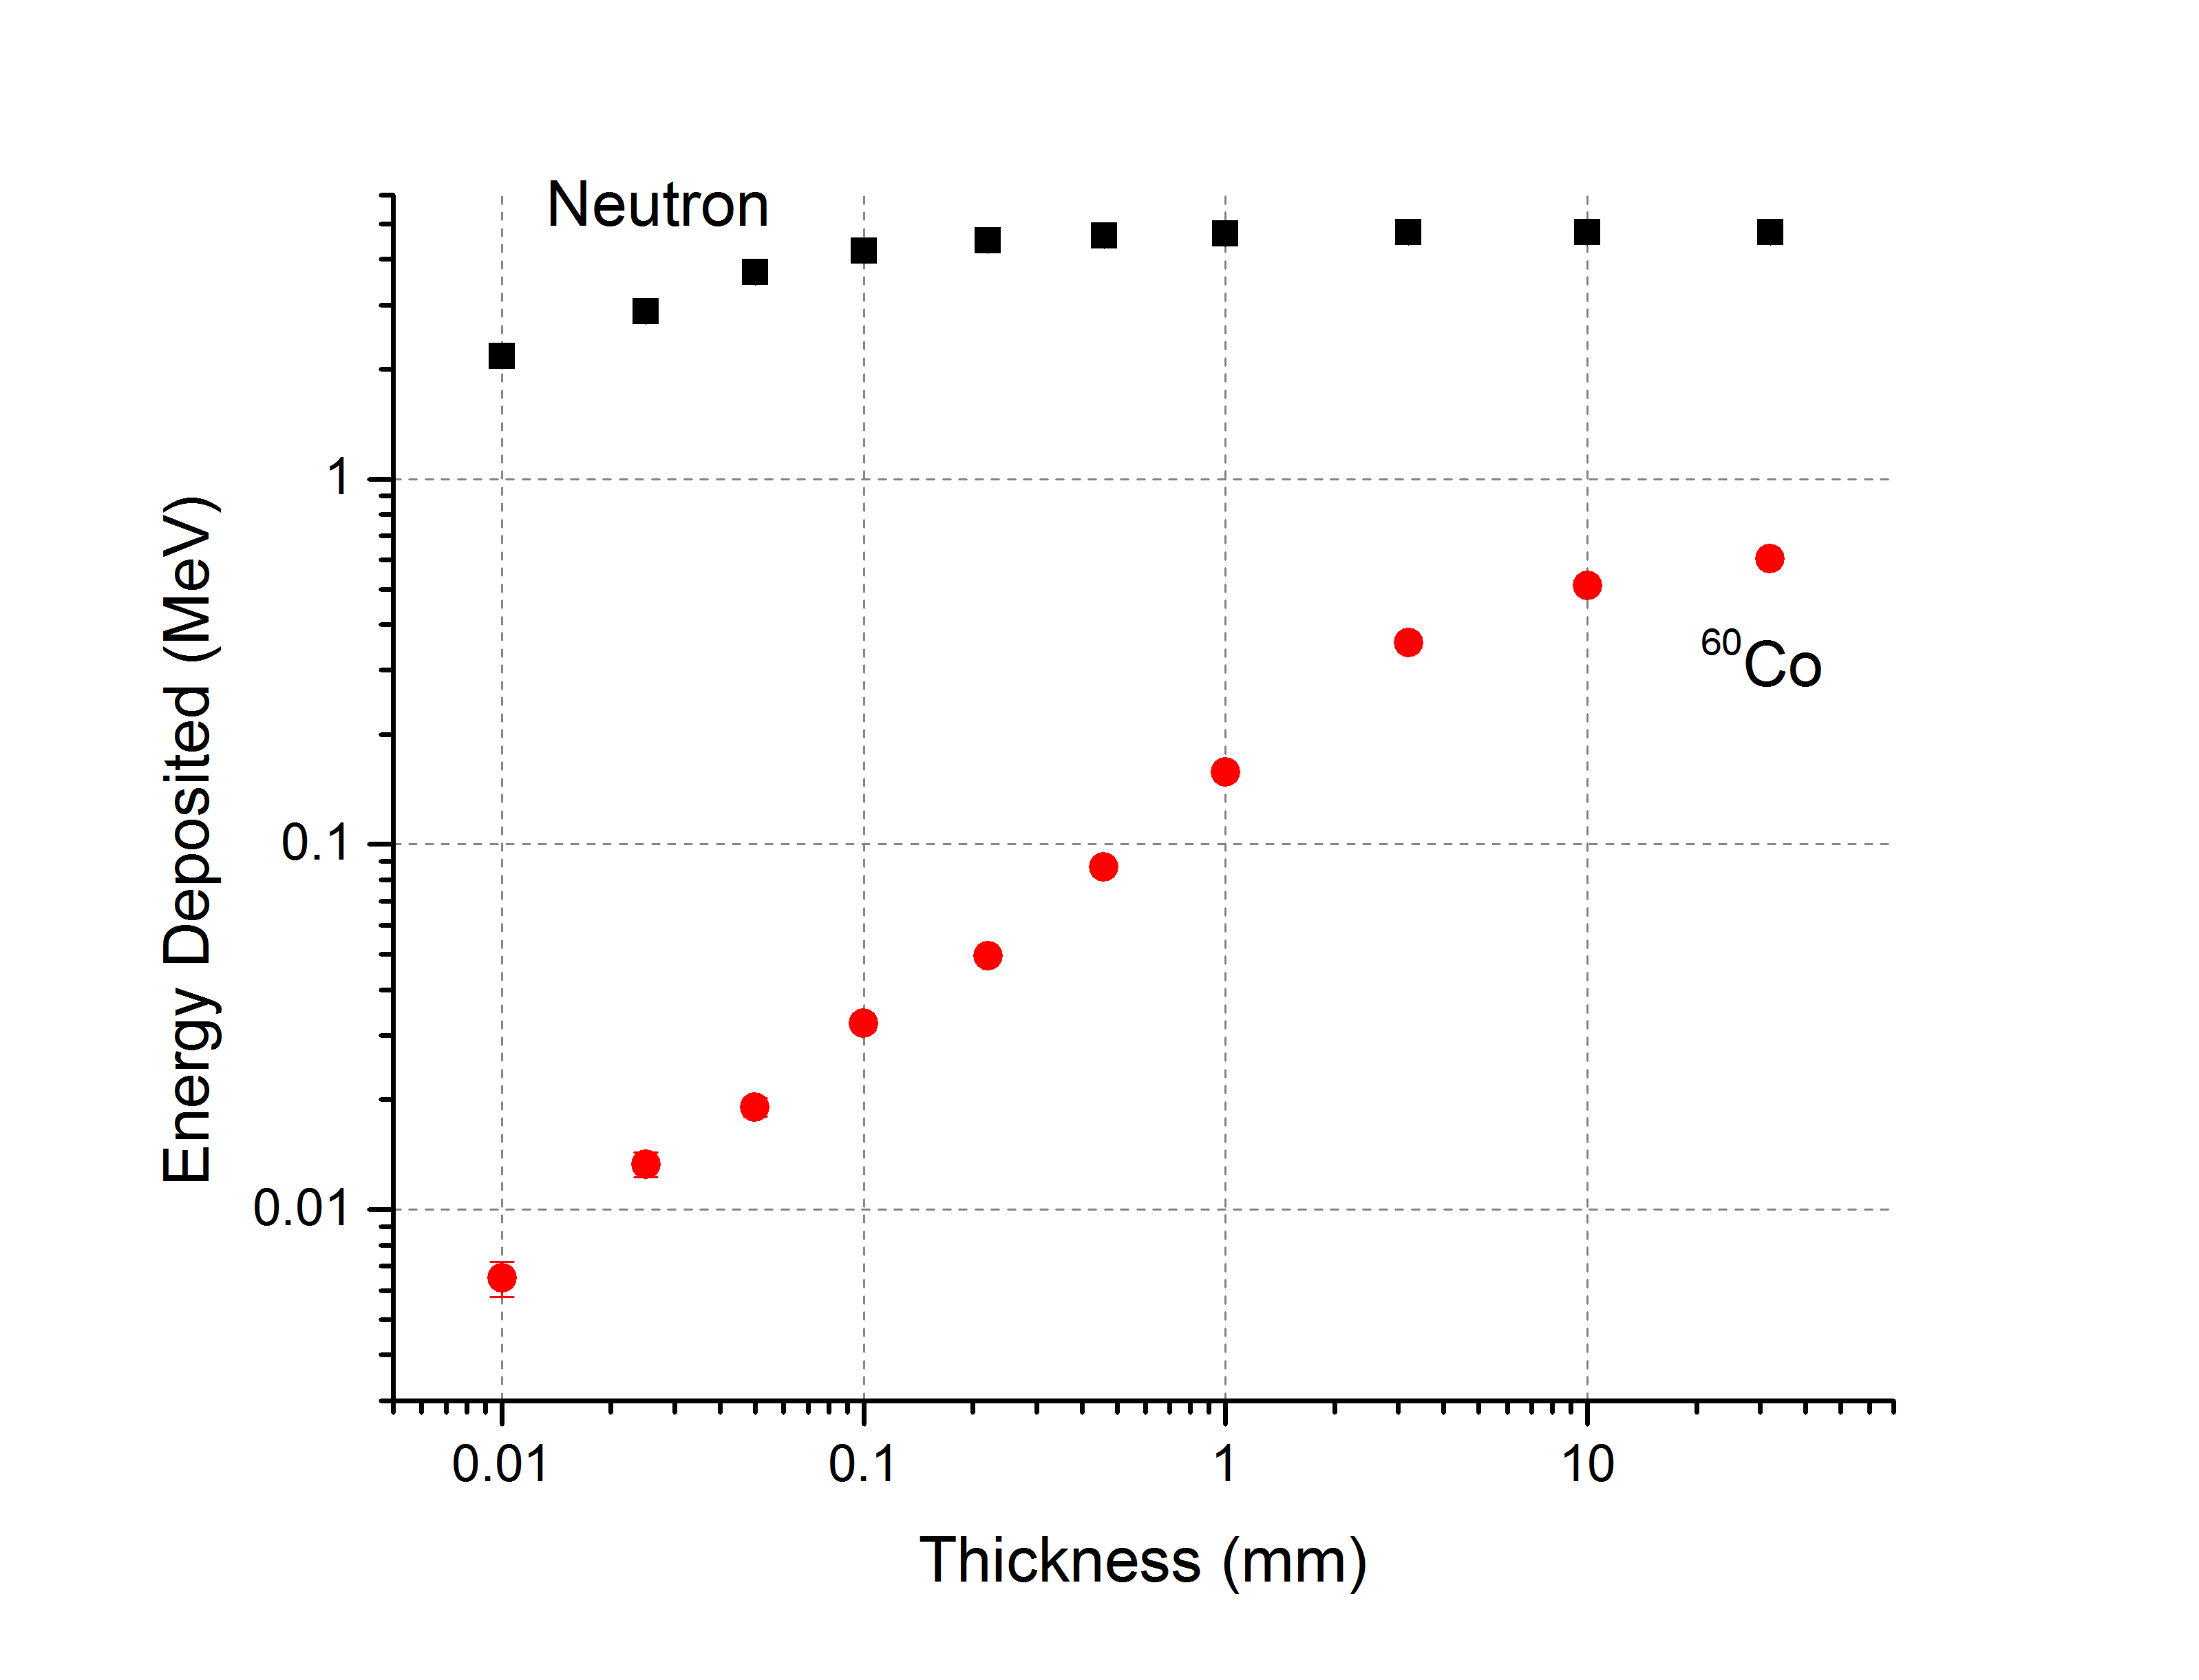
\includegraphics[width=0.6\textwidth]{SimulatedEnergyDeposition}
  \caption[Simulated Energy Deposition and Film Thickness]{Simulated energy deposition and film thickness.  As the films get much thinner it is very unlikely for gamma events to deposition all of their energy, while above \SI{50}{\um} there is very little impact on the energy deposited by neutrons.}
  \label{fig:SimEDep}
\end{figure}

\begin{figure*}[ht]
	\centering
	\begin{subfigure}[b]{0.45\textwidth}
    		\includegraphics[width=\textwidth]{{posEDepCo600.025}.png}
		\caption{ \SI{25}{\um} Gamma (\iso[60]{Co})}
	\end{subfigure}%
	~
	\begin{subfigure}[b]{0.45\textwidth}
    		\includegraphics[width=\textwidth]{{posEDepCo6010.0}.png}
		  \caption{ \SI{1}{\cm} Gamma (\iso[60]{Co})}
	\end{subfigure}%
	
  \begin{subfigure}[b]{0.45\textwidth}
    		\includegraphics[width=\textwidth]{{posEDepneutron0.025}.png}
		\caption{ \SI{25}{\um} Neutron}
	\end{subfigure}%
	~
	\begin{subfigure}[b]{0.45\textwidth}
    		\includegraphics[width=\textwidth]{{posEDepneutron10.0}.png}
		  \caption{ \SI{1}{\cm} Neutron}
	\end{subfigure}%
	\caption[Simulated Energy Deposition and Position]{Simulated average energy depositions and the position of the first interactions. The beam is considered to be incident on position 0, and thus interactions that occur on the front of the film have a much higher probability depositing all of their energy. Events that occur on the edge of the film much less likely to deposit all of their available energy.}
	\label{fig:EDepPosSim}
\end{figure*}

\autoref{fig:simKinE} illustrates the simulated kinetic energy of secondary electrons from Compton scattering and from alpha and triton interactions.
It is observed that kinetic energy of the secondary electrons from the neutron reaction products have predominately energies in the kilo-volt range, while the Compton scattering electrons have energies in hundreds of kilo-volts range. 
However, it should be noted that there is only one secondary electron from a Compton scattering and multiple secondary electrons from the reaction products.
\autoref{fig:ReacProdDist} shows the distribution of the number of secondary electrons from the alpha and triton and their kinetic energy.
\begin{figure}[ht]
    \centering
    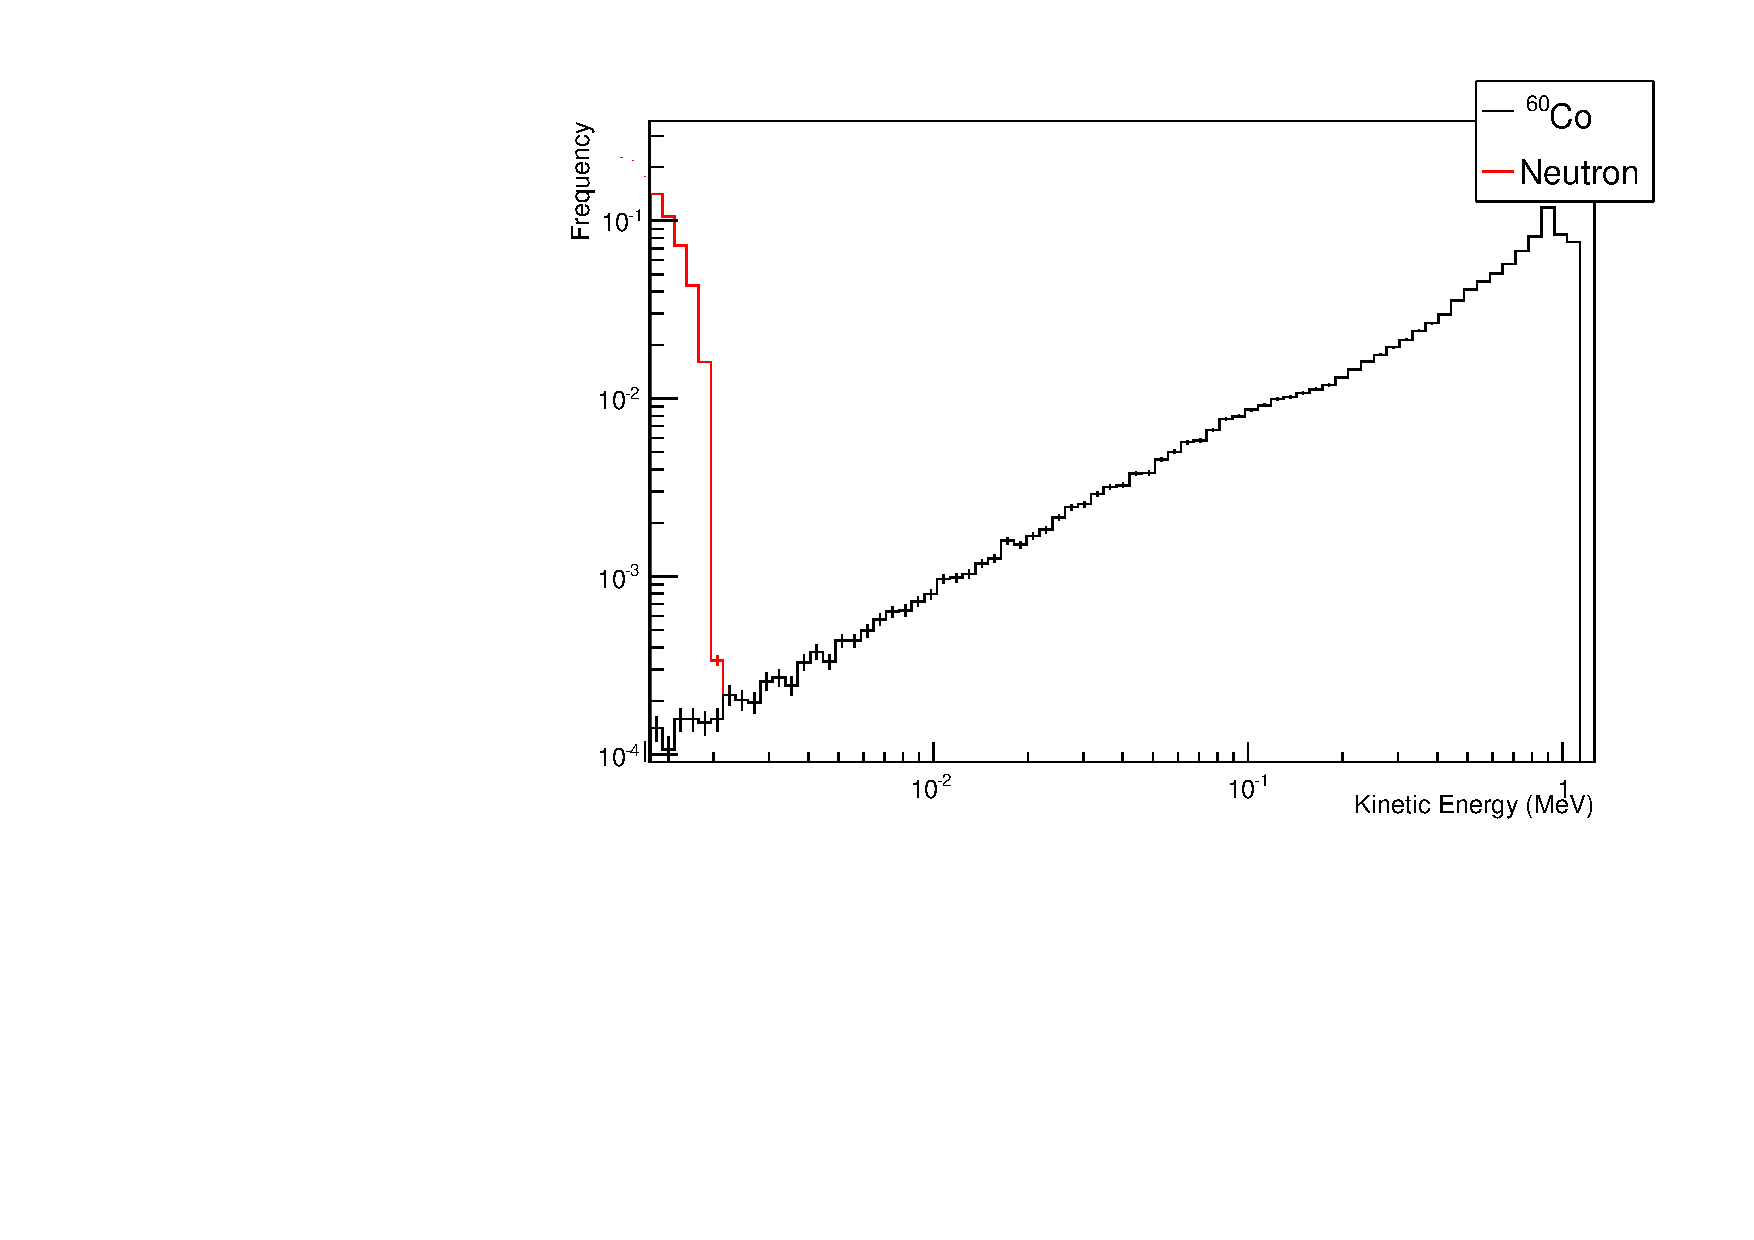
\includegraphics[width=\textwidth]{NGSecElecKinEDist}
    \caption{Simulated Kinetic Energy of Secondary Electrons from Compton Scattering and from \iso[6]{Li} reaction products}
    \label{fig:simKinE}
\end{figure}
\begin{figure*}[ht]
	\centering
	\begin{subfigure}[b]{0.45\textwidth}
    		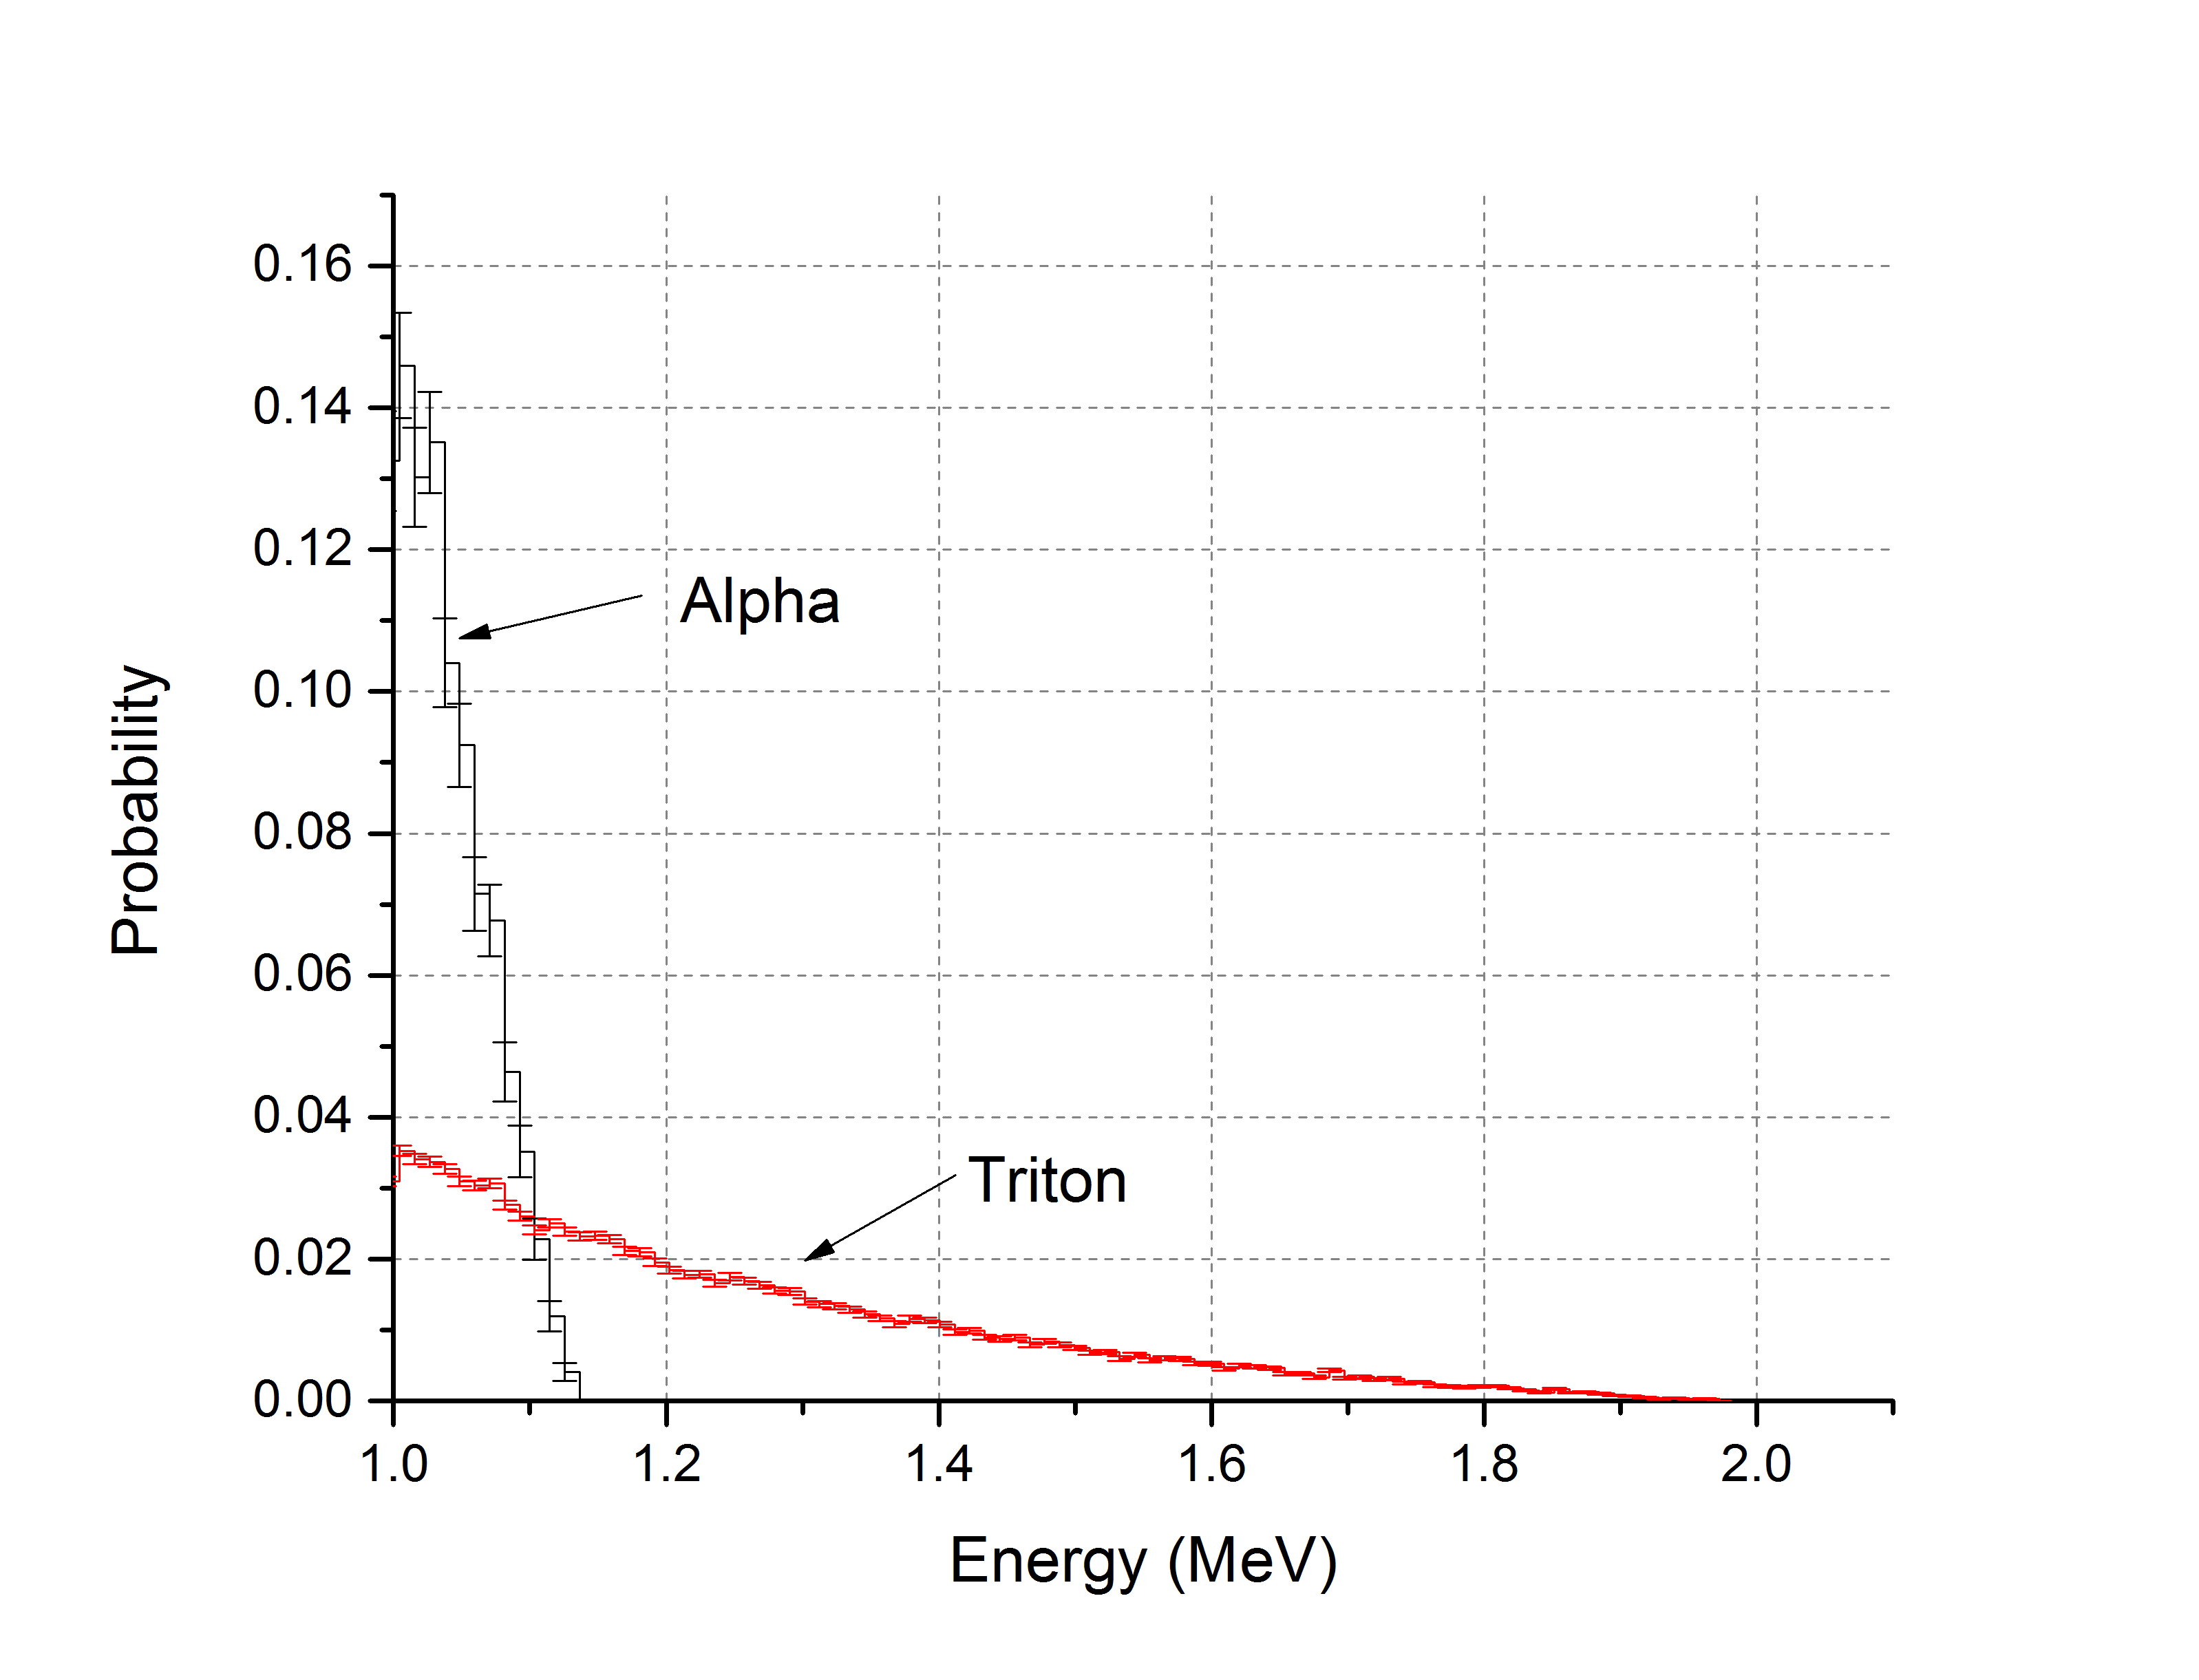
\includegraphics[width=\textwidth]{AlphaTritonSecElecKinEDist}
		\caption{Alpha and Triton Secondary Electron Kinetic Energy Distribution}
	\end{subfigure}%
	~
	\begin{subfigure}[b]{0.45\textwidth}
    		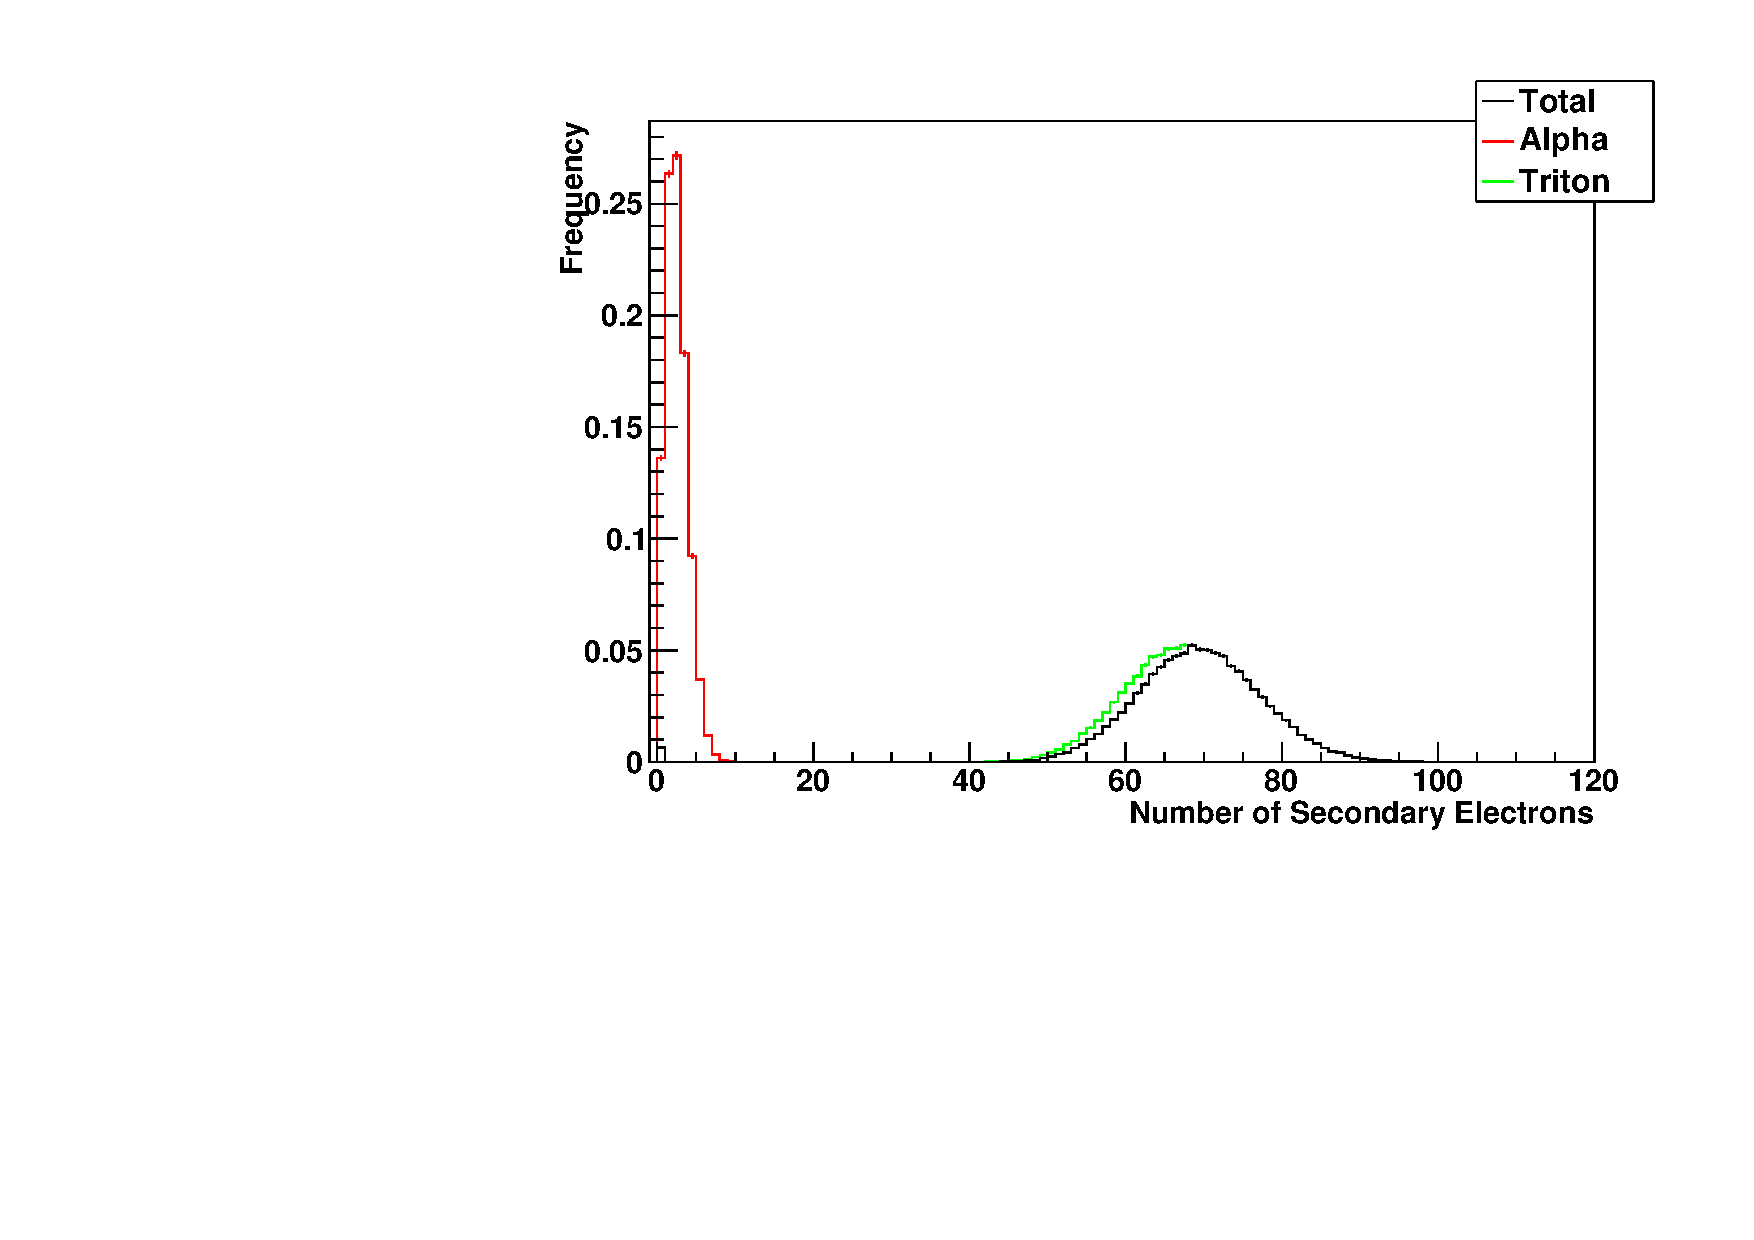
\includegraphics[width=\textwidth]{NeutronNumSecElec}
		\caption{Number of Secondary Electrons Produced Per Neutron Interaction}
	\end{subfigure}%
	\caption{Neutron Reaction Products Secondary Electrons Energies}
	\label{fig:ReacProdDist}
\end{figure*}
%%%%%%%%%%%%%%%%%%%%%%%%%%%%%%%%%%%%%%%%%%%%%%%%%%%%%%%%%%%%%%%%%%%%%%%%%%%
%                                                                         %
%                  Light Yield and Energy Deposition                      %
%                                                                         %
%%%%%%%%%%%%%%%%%%%%%%%%%%%%%%%%%%%%%%%%%%%%%%%%%%%%%%%%%%%%%%%%%%%%%%%%%%%
\section{Light Yield and Energy Deposition}
The energy deposition and light yield were also investigated by simulations in the GEANT4 environment for polystyrene based films (light output 1,000 photons per MeV).
These simulations (summarized in \autoref{fig:EDepLightYield}) show that as expected the light output was linear with the energy deposition.
\begin{figure*}[ht]
	\centering
	\begin{subfigure}[b]{0.45\textwidth}
    		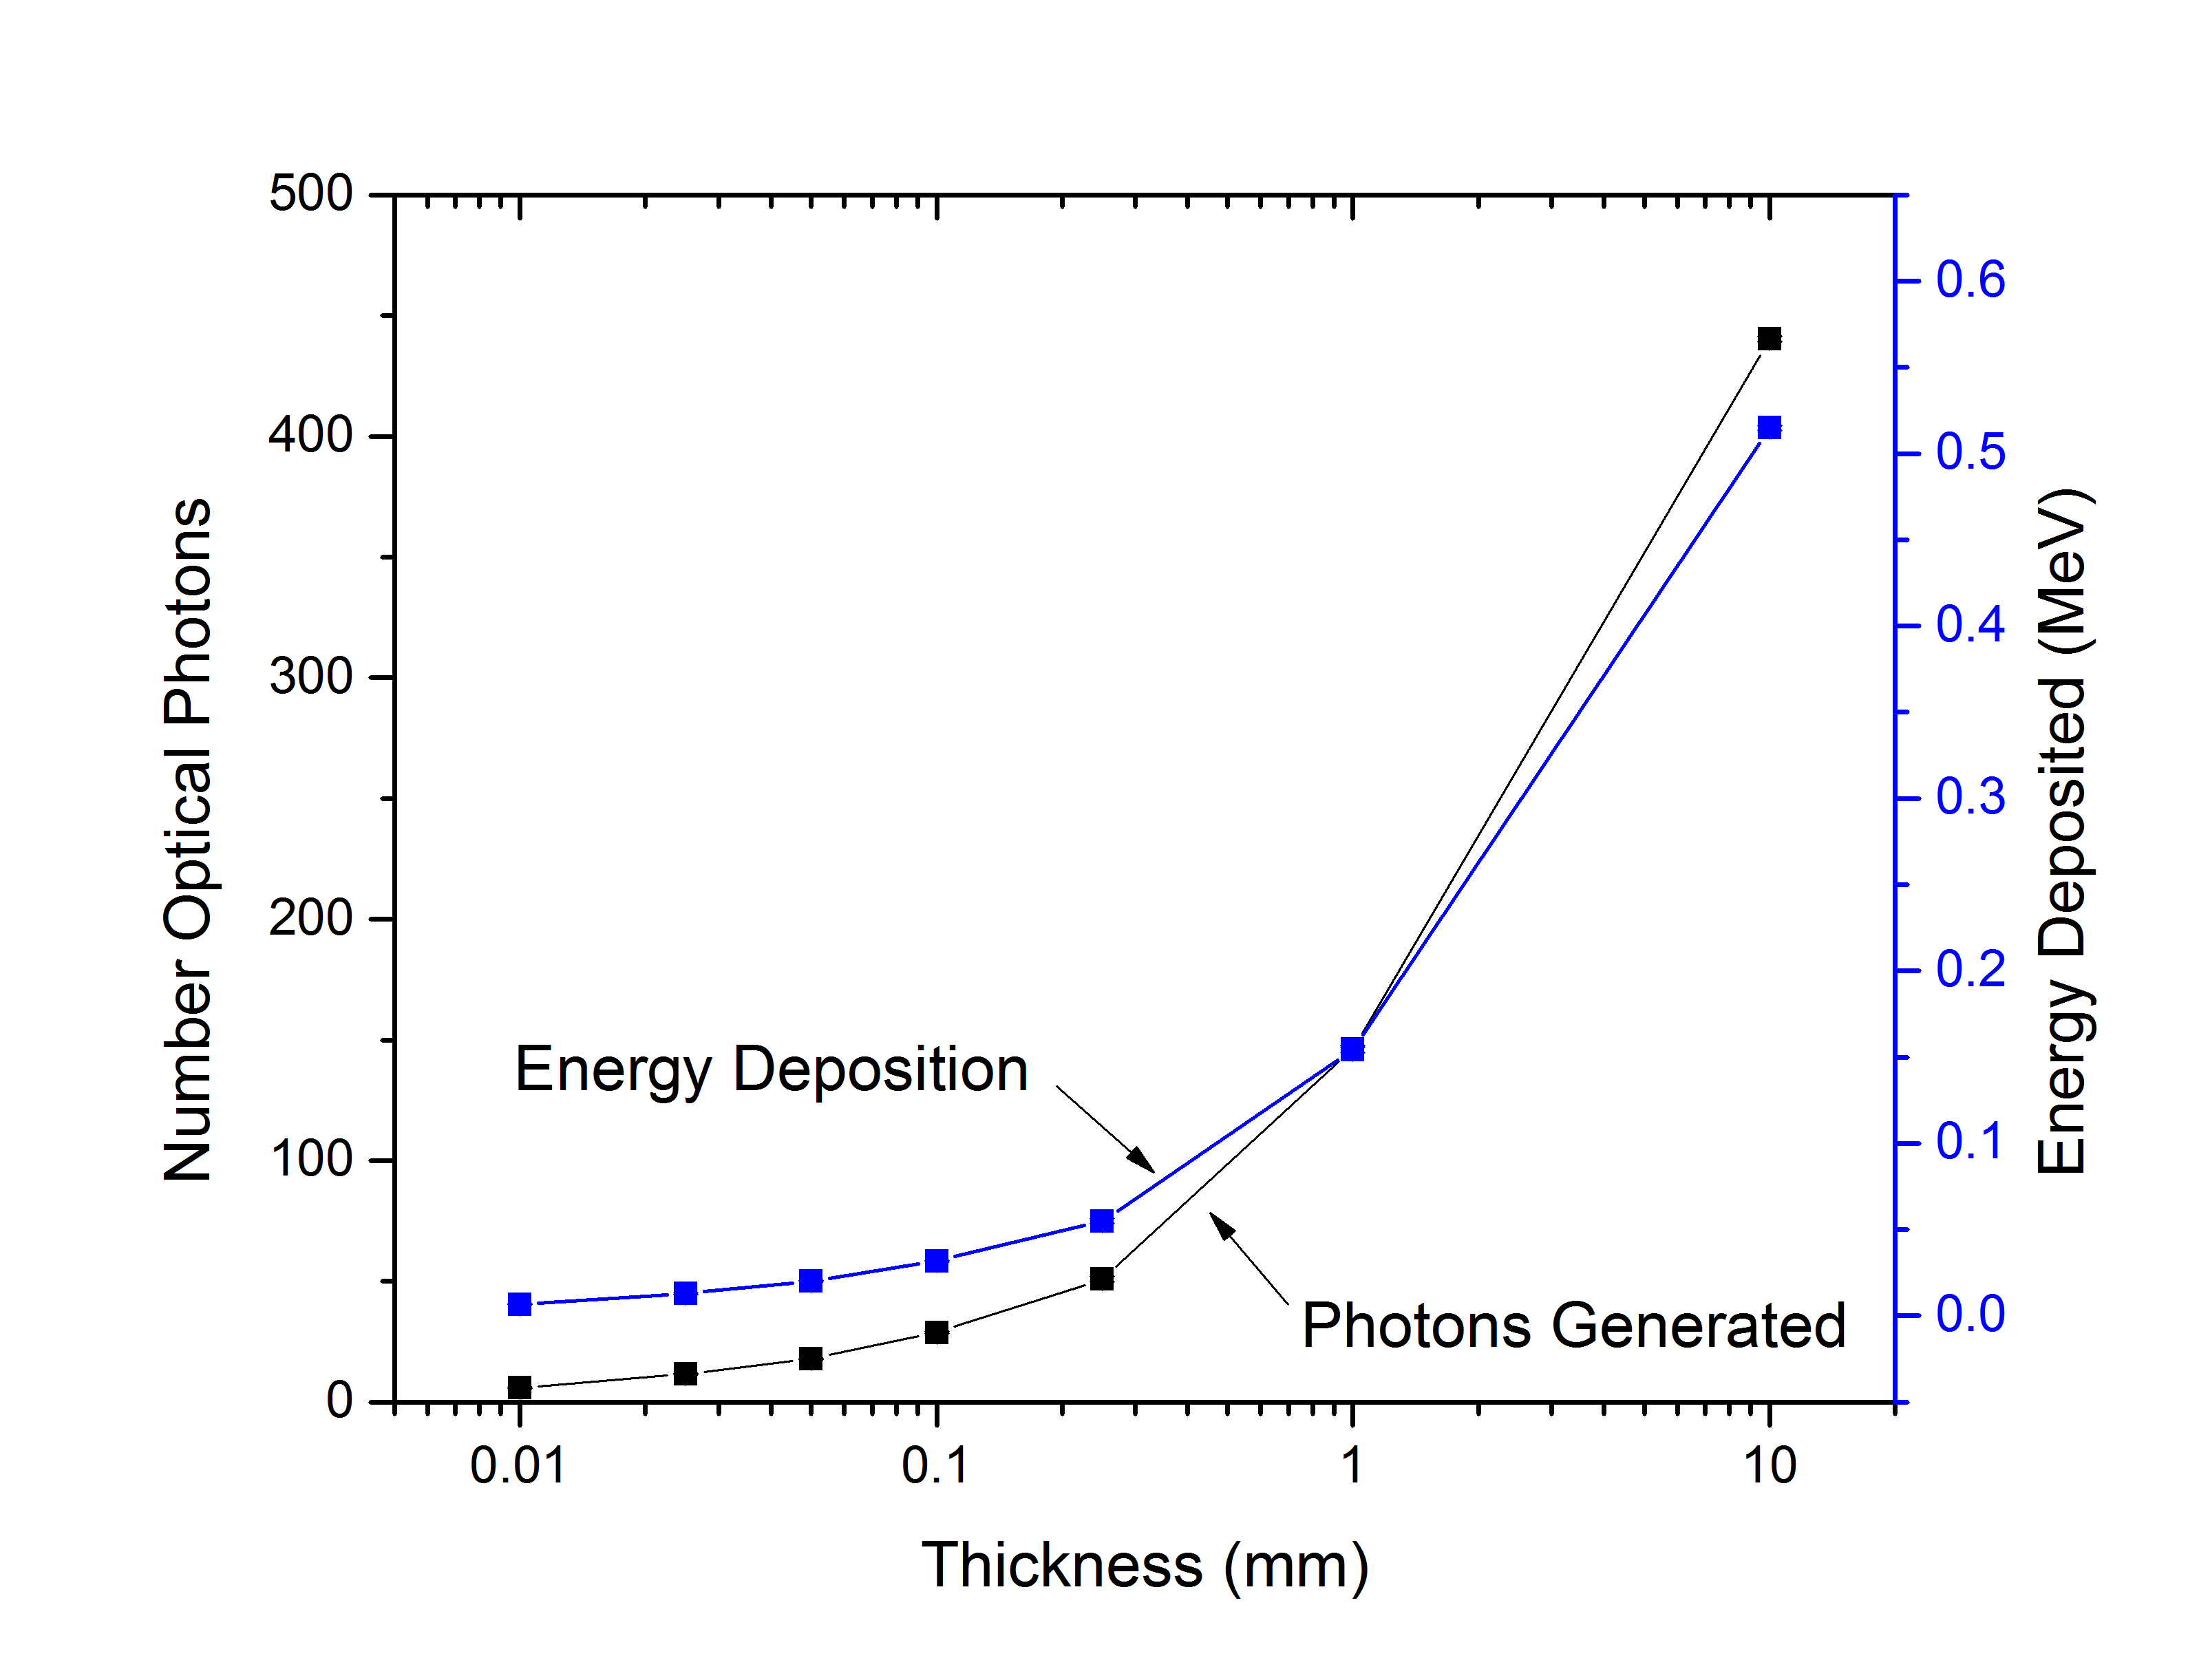
\includegraphics[width=\textwidth]{EDepLightYield_Gamma}
		\caption{ Gamma (\iso[60]{Co}}
	\end{subfigure}%
	~
	\begin{subfigure}[b]{0.45\textwidth}
    		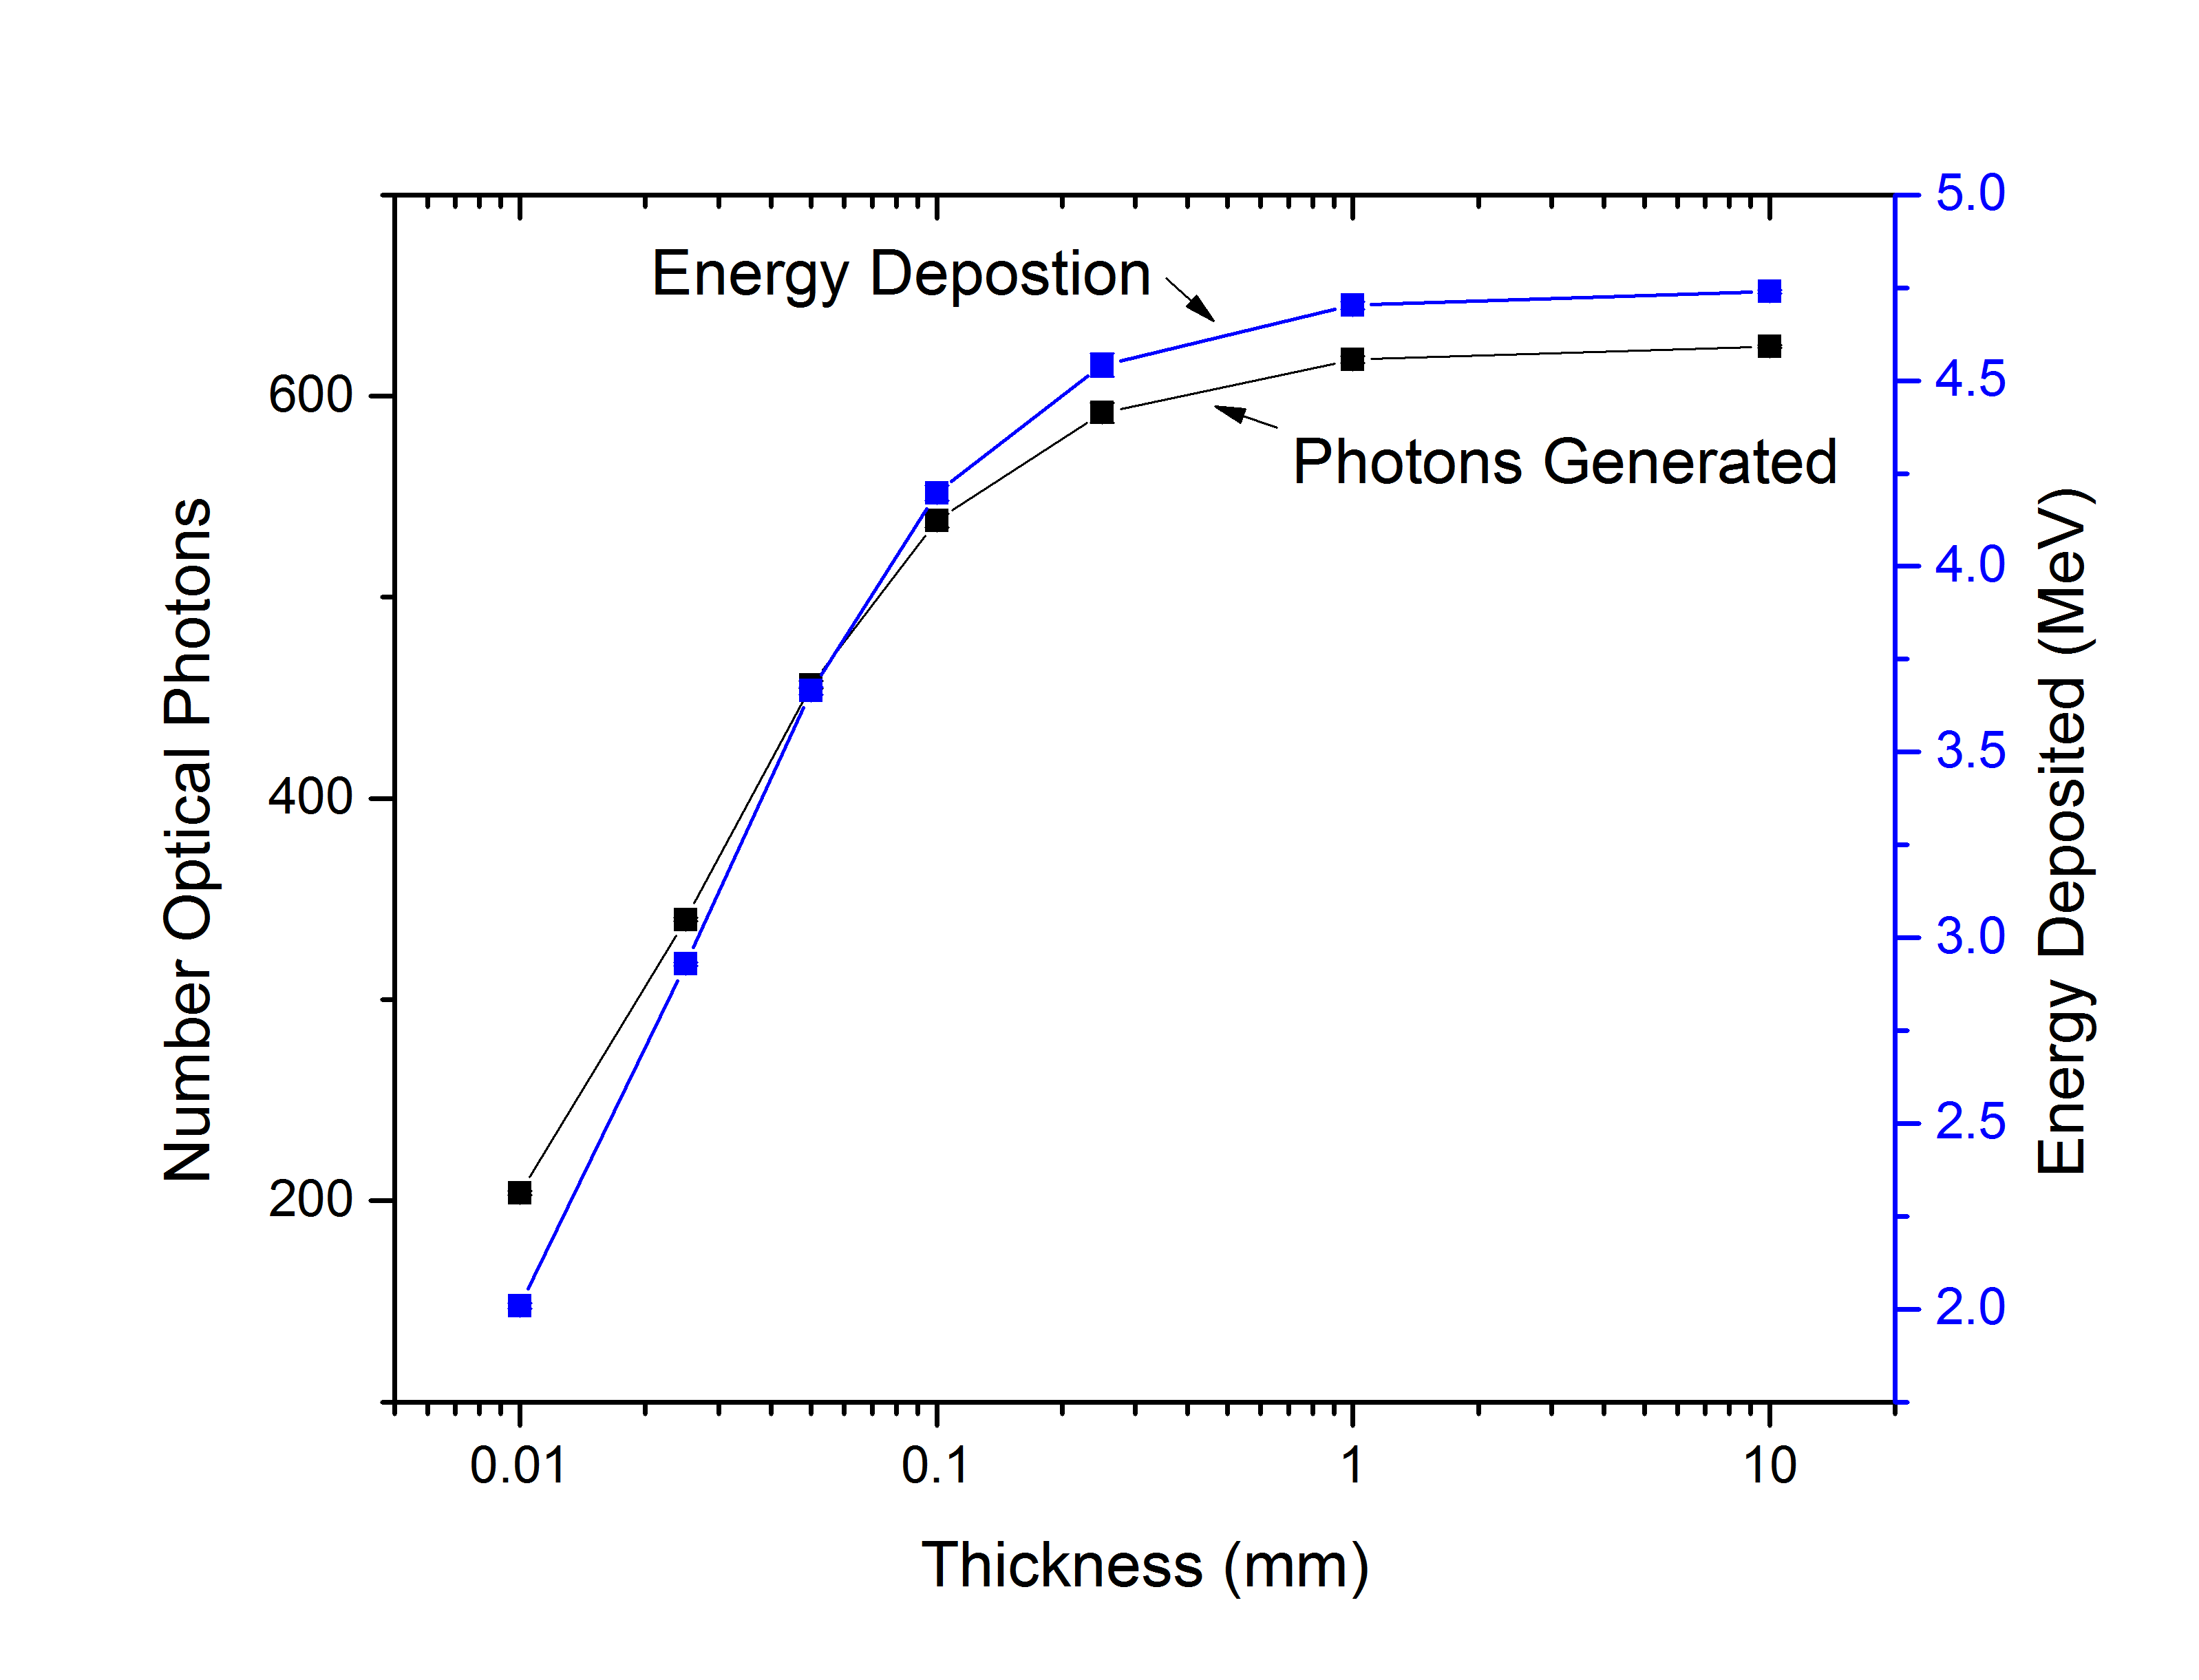
\includegraphics[width=\textwidth]{EDepLightYield_Neutron}
		  \caption{ Neutron}
	\end{subfigure}%
  \caption[Energy Deposition and Light Yield]{Simulated energy deposition and light yield.  The light yield is fairly linear with the energy deposition, thus, the energy deposition is an adequate indicator of the expected light yield.}
  \label{fig:EDepLightYield}
\end{figure*}
However, it is instructive to look at the distributions of how many photons were created per event.
As the films become thicker and more of the triton energy is captured the response of the triton starts to dominate the alpha (\autoref{fig:NeutronPhotonsGenSim}), resulting in the number of photons peaking around around 650 photons for this simulated sample.
For photons, shown in \autoref{fig:GammaPhotonsGenSim}, it is observed that the distribution is flat for very thick films, but for thinner films the probability is greatly increased for an event to generate a low number of photons.
\begin{figure}
  \centering
  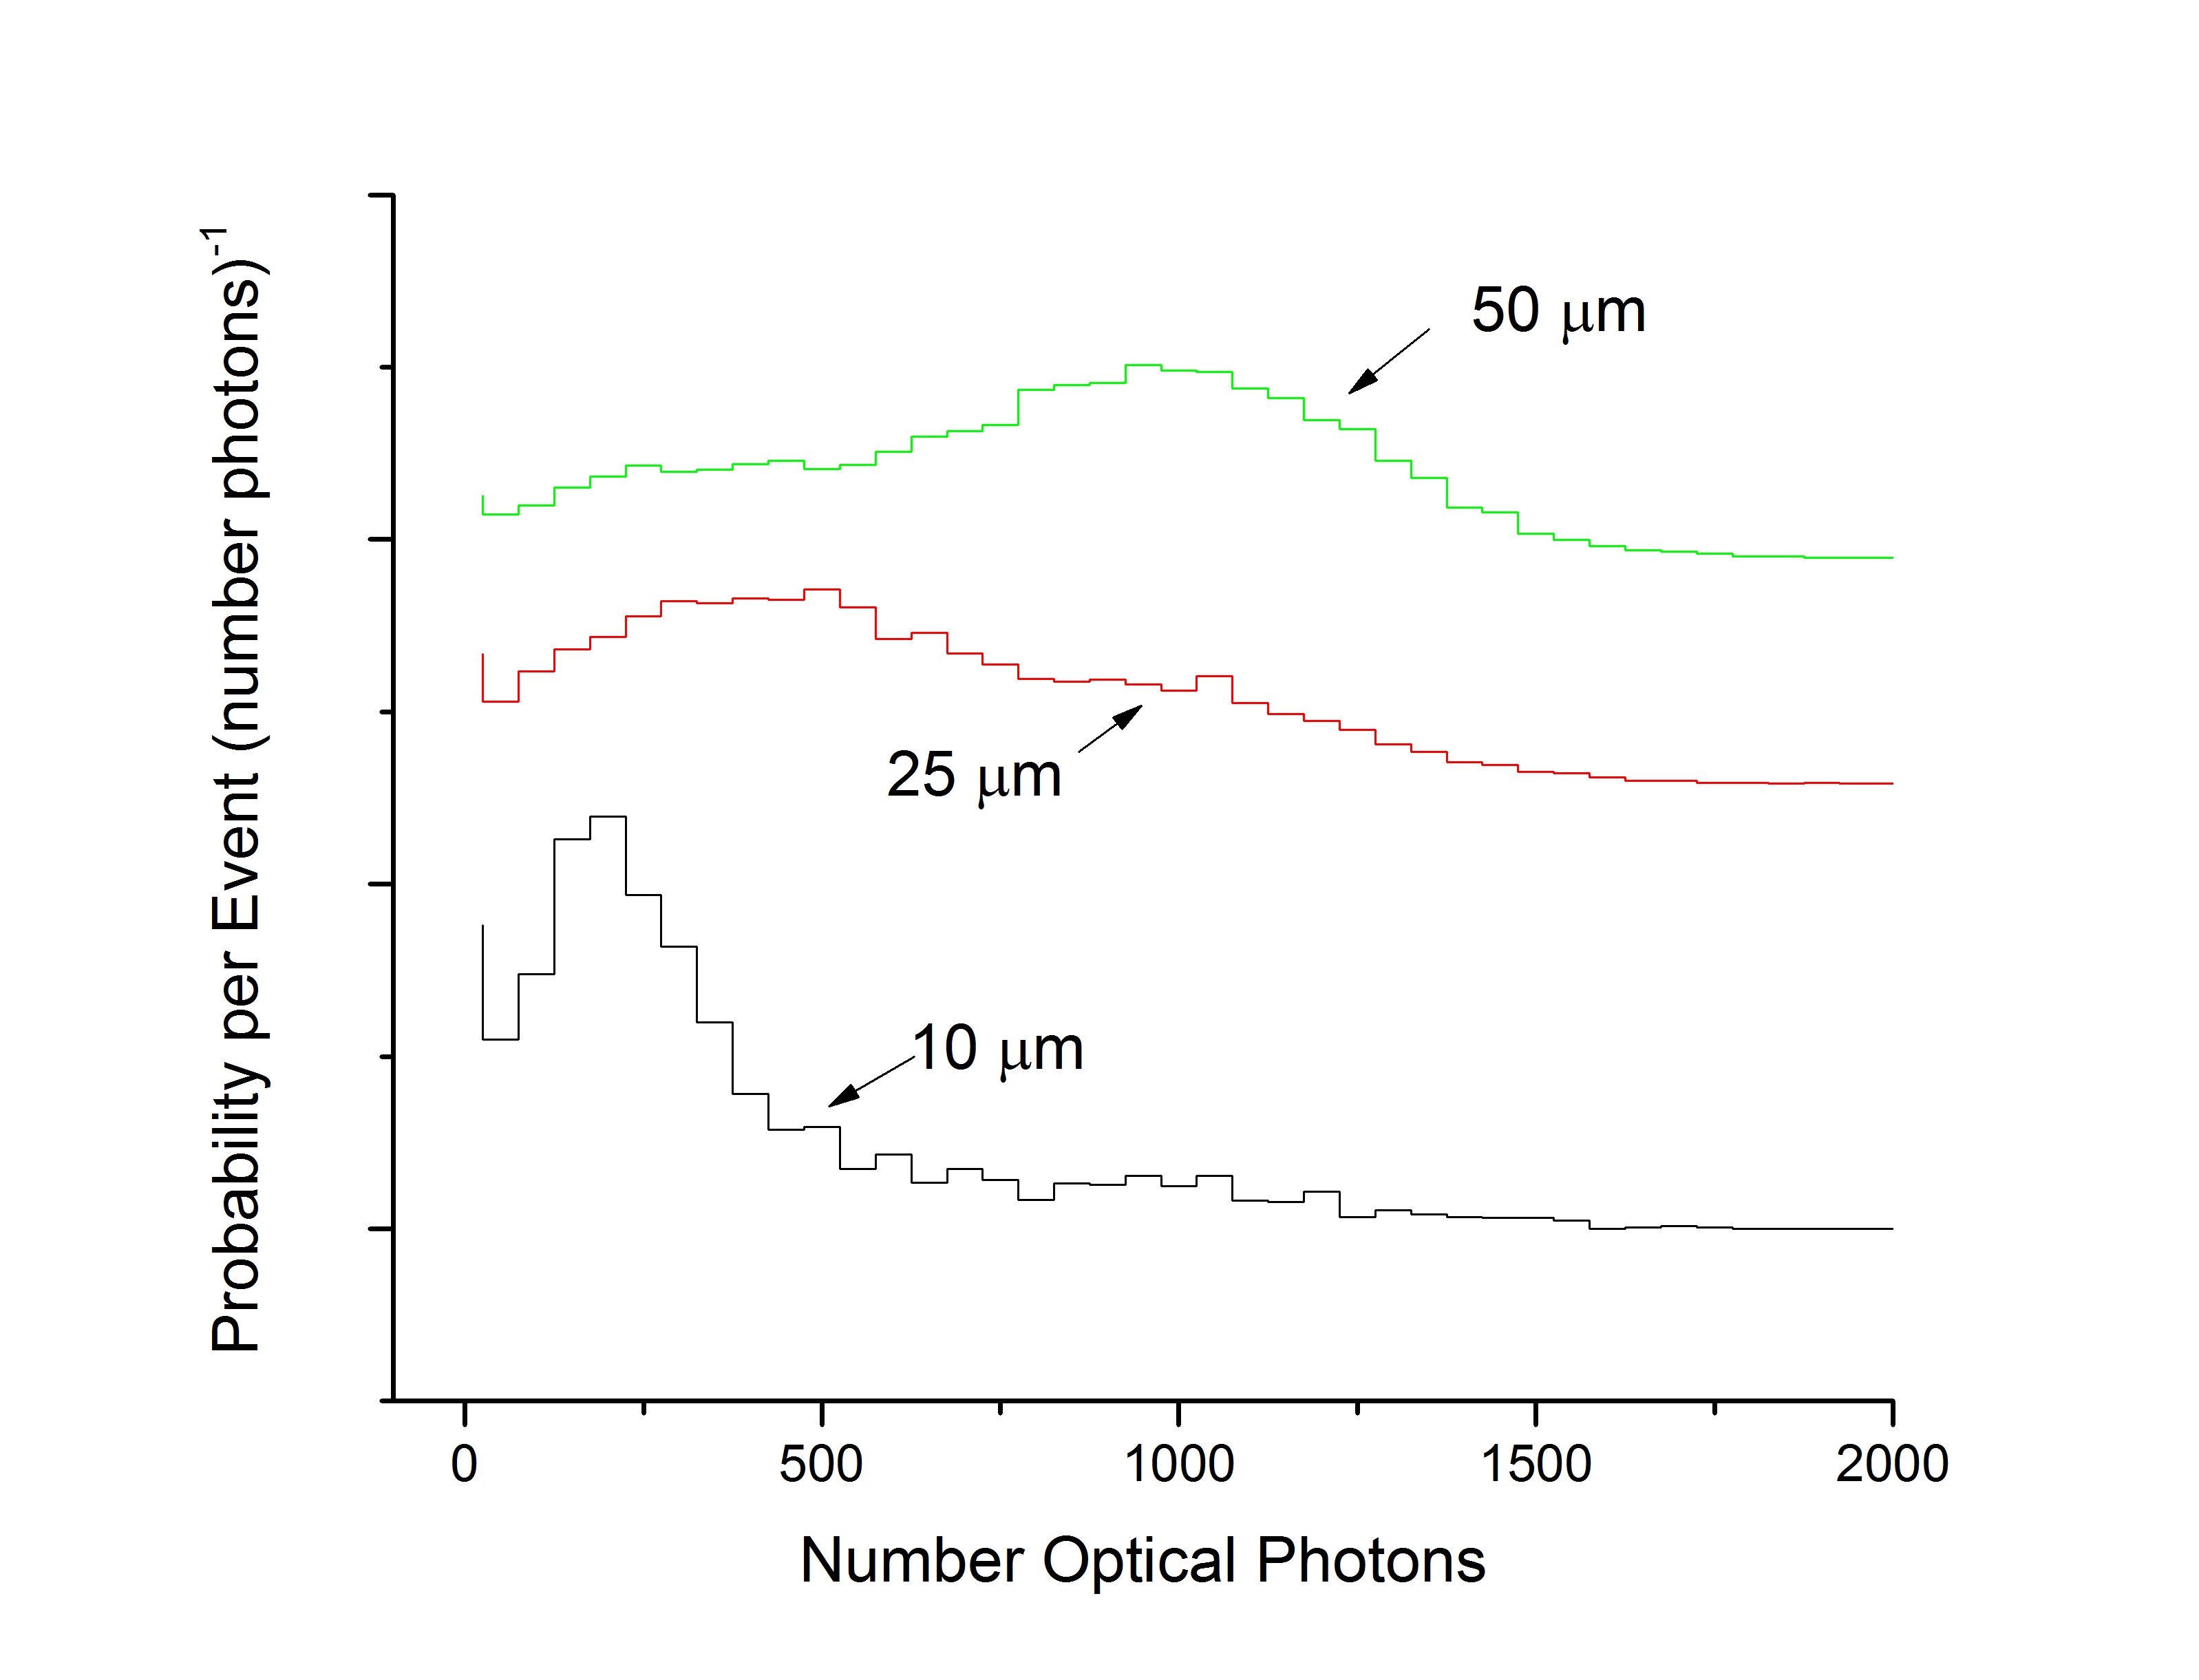
\includegraphics[width=\textwidth]{Neutron_PhotonsGenerated_Sim}
  \caption[Number of photons generated from neutron interactions]{Simulated number of photons generated from neutron interactions.  For the \SI{10}{\um} film it is observed that the majority of the photons are generated by a partial energy deposition corresponding to the alpha particle, and this effect tappers off as the films get thicker}
  \label{fig:NeutronPhotonsGenSim}
\end{figure}
\begin{figure}
  \centering
  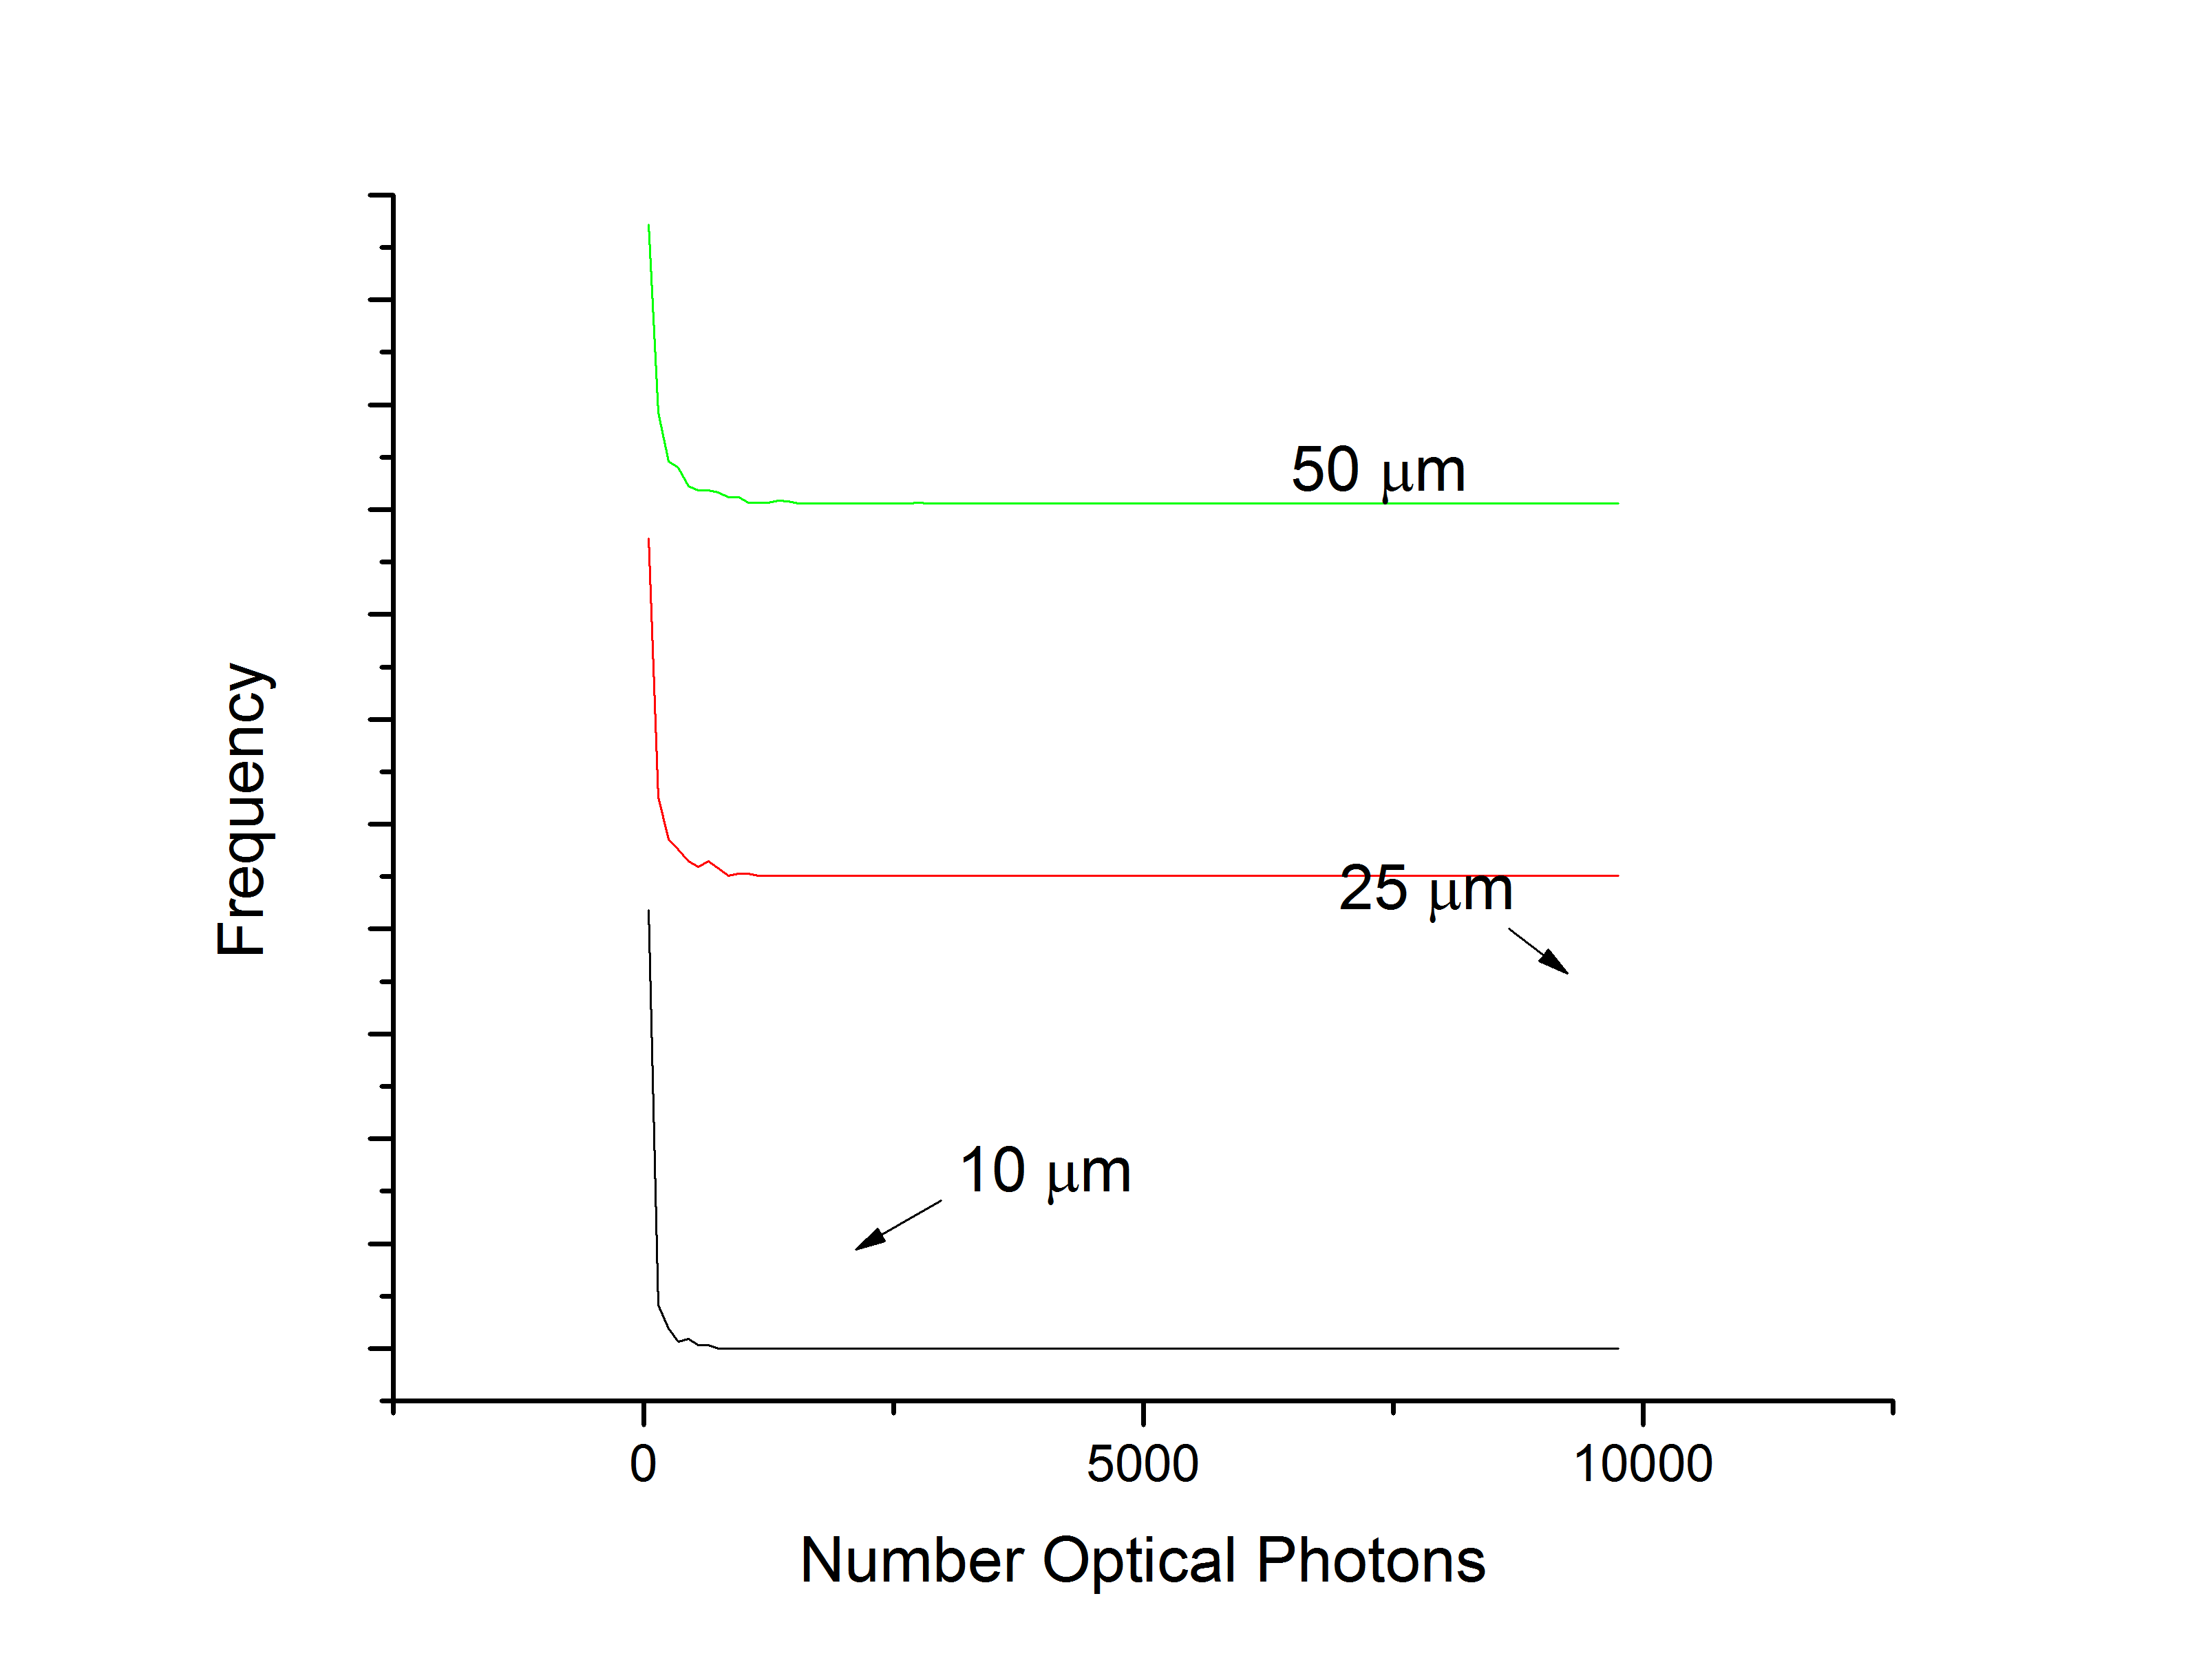
\includegraphics[width=\textwidth]{Gamma_PhotonsGenerated_Sim}
  \caption[Number of photons generated from gamma interactions]{Simulated number of photons generated from gamma interactions.}
  \label{fig:GammaPhotonsGenSim}
\end{figure}
\begin{figure}
  \centering
  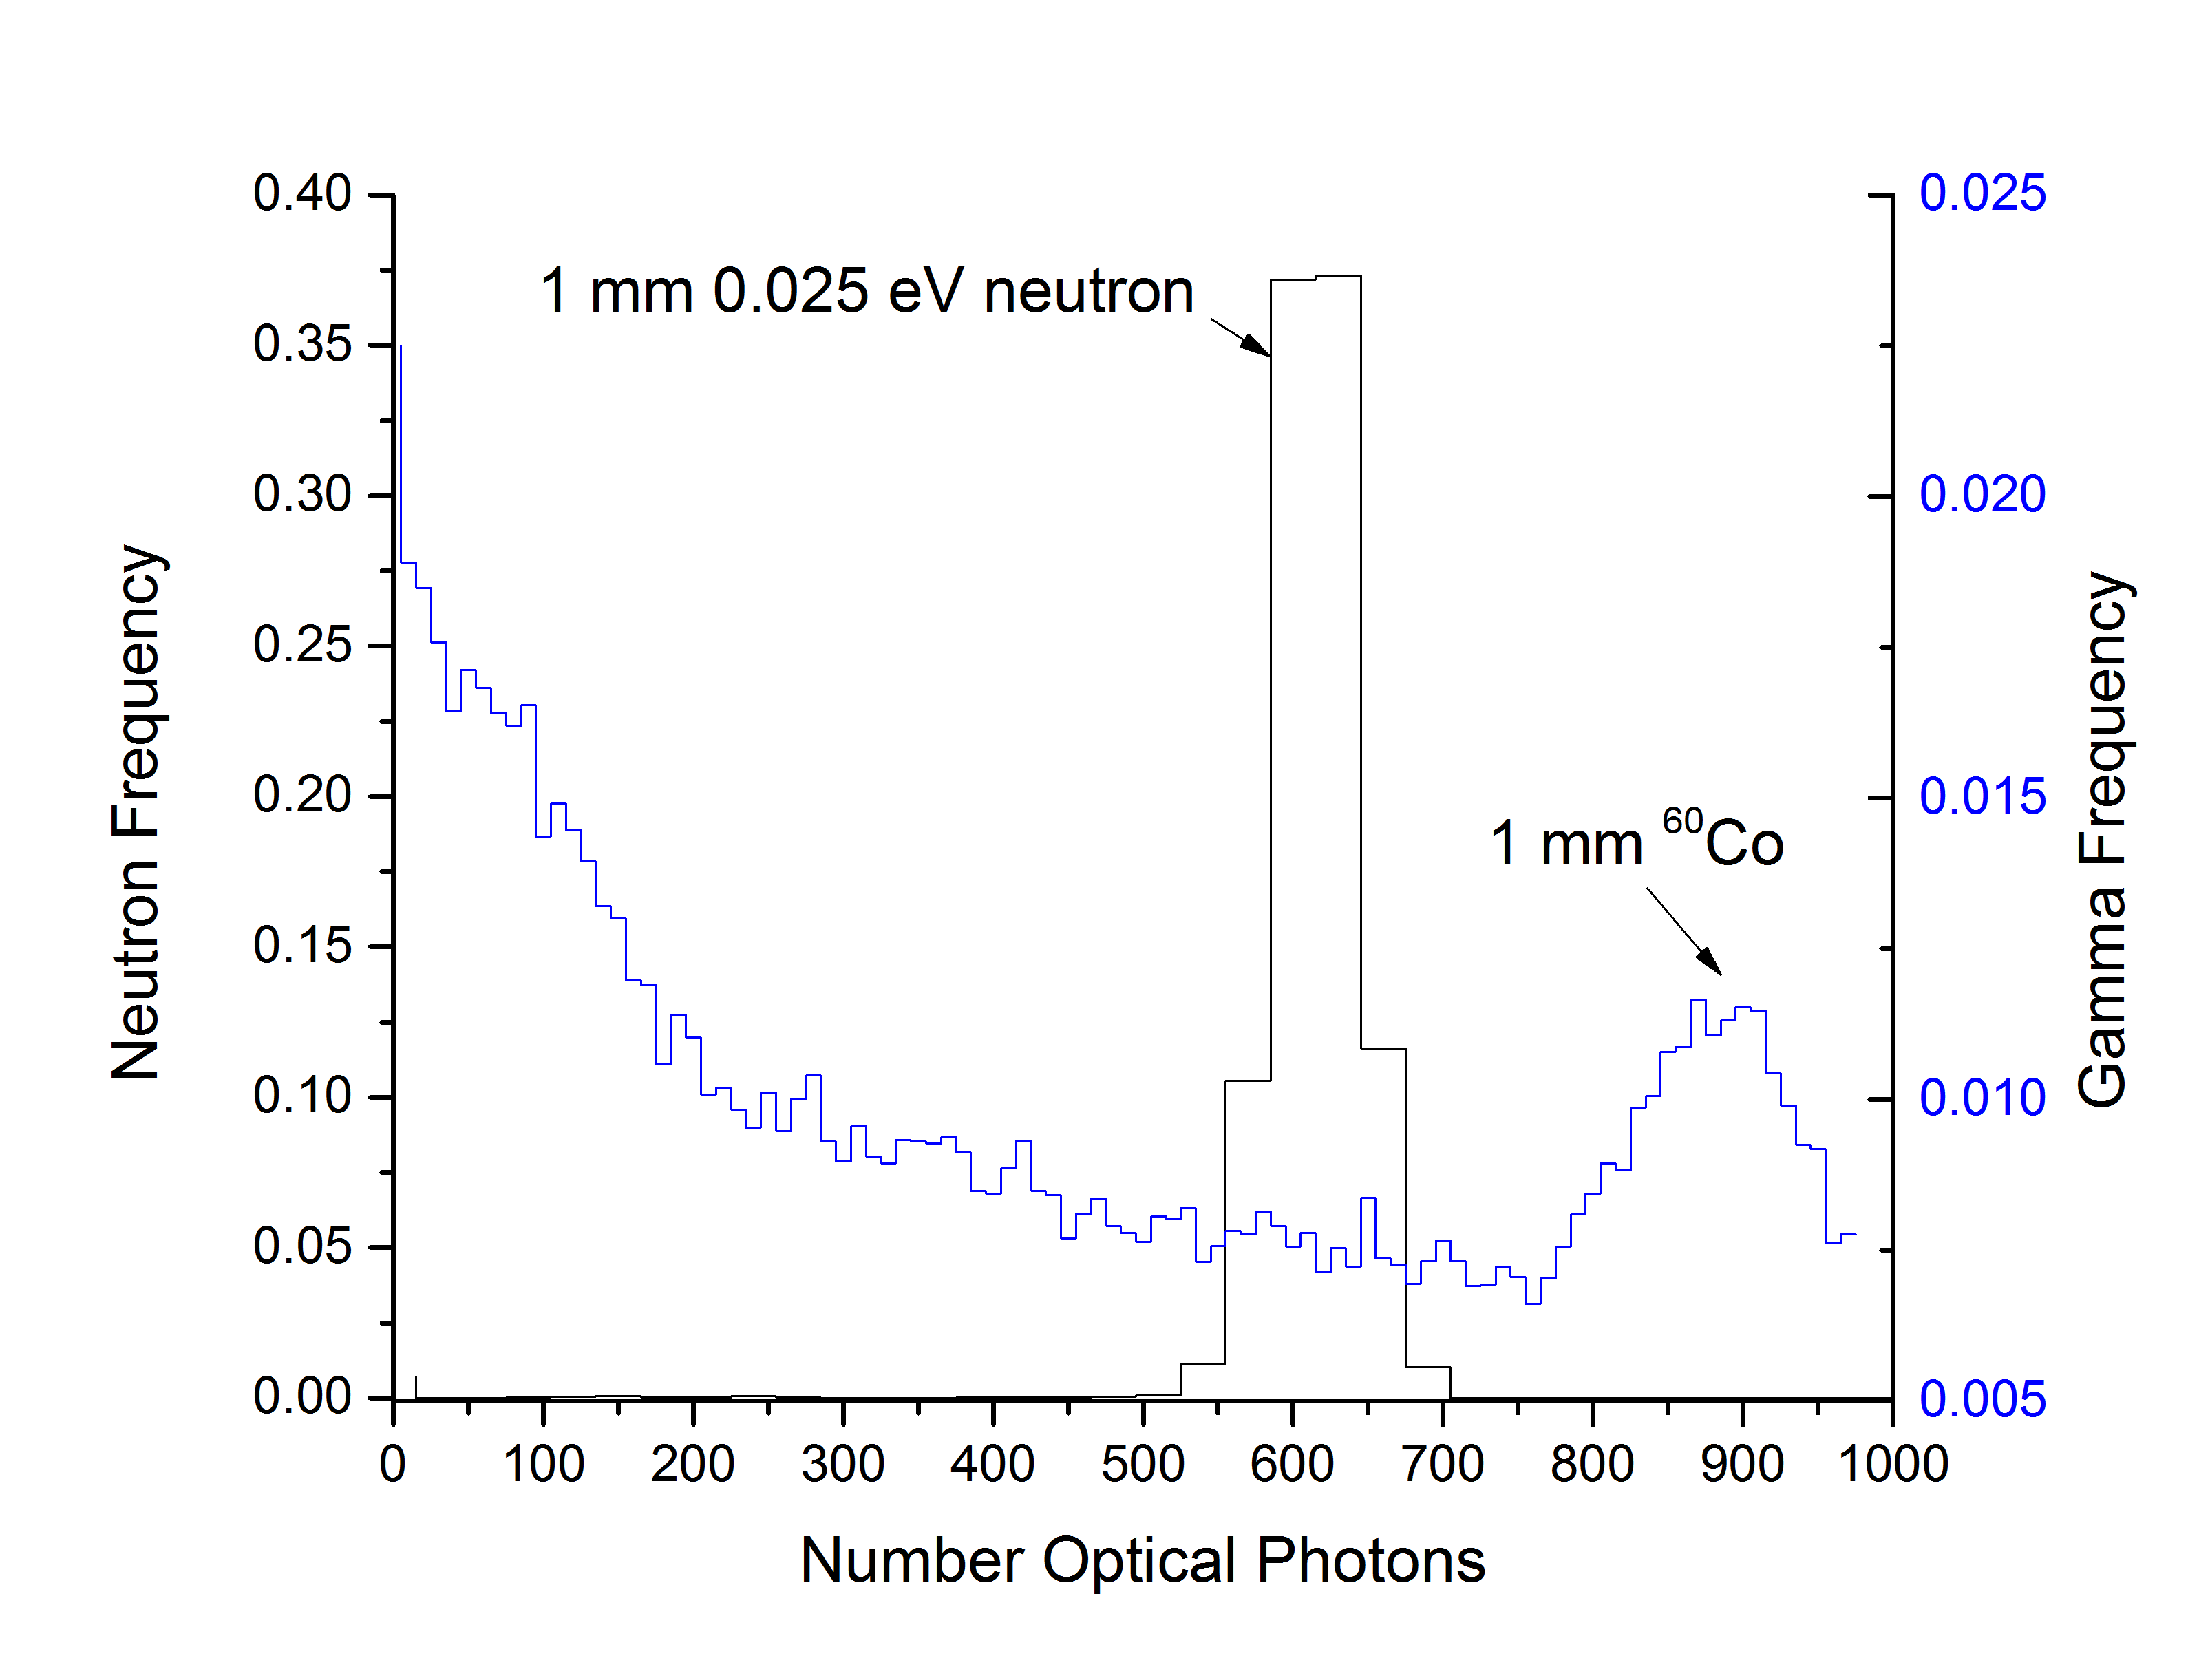
\includegraphics[width=\textwidth]{NeutronGamma_PhotonsGenerated_Sim}
  \caption[Number of photons generated of a 1 mm for neutron and gamma interactions]{Simulated number of photons generated from neutron and gamma interactions.}
  \label{fig:NeutronGammaPhotonsGenSim}
\end{figure}
%%%%%%%%%%%%%%%%%%%%%%%%%%%%%%%%%%%%%%%%%%%%%%%%%%%%%%%%%%%%%%%%%%%%%%%%%%%
%                                                                         %
%                      Pulse Height Discrimination                        %
%                                                                         %
%%%%%%%%%%%%%%%%%%%%%%%%%%%%%%%%%%%%%%%%%%%%%%%%%%%%%%%%%%%%%%%%%%%%%%%%%%%

\section{Pulse Height Dissemination}
\label{sec:PulseHeightDiscrm}
The criteria set forth by the DHS-DNDO require that all replacement portal monitors have an intrinsic gamma-ray efficiency of less than one in a million.
Simply put, for a million photons that pass through the detector only a single one of those can be considered as a count.
One such technique for achieving a gamma ray intrinsic efficiency is to set a pulse height discriminator setting such that pulse below that discriminator are discarded.
The basis for setting a pulse height discriminator to differentiate between neutron and gammas can be attributed to the secondary electrons and the difference in energy mechanisms as presented in the first section of this chapter.
However, the application to physical detectors has yet to be concretely formulated.
This section will serve to remedy that and present a pulse height discrimination scheme capable of discrimination between neutrons and gammas.

A pulse height discriminator is usually set by the hardware electronics, but need not be a physical voltage cutoff - it can also be set by software in an offline analysis.
A mathematical lower level discriminator (MLLD) is then introduced to clarify the determination of what discriminator setting will be necessary to achieve a given intrinsic efficiency criteria.
The intrinsic efficiency for a given MLLD is determined for a sample by first determining the photon fluence over the sample (usually by a MCNPX calculations, these calculations are explained in \autoref{chap:IntEff}).
The recorded spectra is then normalized the photon fluence to determine the count rate per incident photon per channel.
As the intrinsic efficiency is defined as the count per incident quanta of radiation, the spectra needs to be integrated from the channel number represented by the MLLD to the end of the spectra over the channels to determine the count rate.
By summing only the counts that are above the discriminator represented as the MLLD these counts are then discarded from the analysis.
A formulation of the MLLD is presented in \eqref{eqn:MLLDFormulation},
\begin{align}
	\epsilon_{\gamma,int}\left(MLLD\right) &= \frac{\int_{MLLD}^{\infty}p(x)dx}{\Phi}
  \label{eqn:MLLDFormulation}
\end{align},
where \definevar{$p(x)$}{spectra as a function of channel number} and \definevar{$\Phi$} is the incident gamma flux.
By computing the gamma intrinsic efficiency as a function of the MLLD, one only needs to find what MLLD corresponds to having a intrinsic efficiency of less than one in a million.

A sequence of polystyrene films (10\% by weight enriched LiF) were fabricated by Dr. Mabe and analyzed for their ability to achieve different gamma intrinsic efficiencies in the MLLD framework.
These measurements and calculations, presented in \autoref{fig:GammaIntEffMLLD}, demonstrate the utility of the MLLD.
This figure shows, as expected, that increasing the MLLD causes a lower intrinsic efficiency as counts below the MLLD are discarded.
Thicker films, where more energy is deposited and thus produce more photons, require higher MLLD settings in order to achieve the same level of discrimination as their thinner counter parts.
\begin{figure}
  \centering
    \includegraphics[width=\textwidth]{PS_intEffMLLD}
  \caption[Intrinsic efficiency achieved at various discriminator settings]{Gamma intrinsic efficiency versus the pulse height discriminator setting (MLLD) to achieve the corresponding level of discrimination. It is observed that there is a change in the shape of the curves reflecting the increased fraction of energy deposition in thicker films relative to the thinner films.}
  \label{fig:GammaIntEffMLLD}
\end{figure}

Such a scheme will not be without cost, however, as the simulations and measurements indicate there is an overlap between the neutron 
The calculated gamma intrinsic efficiency for six polymeric films along with the neutron response of two of the films in \autoref{fig:GammaIntrNeutronCounts}, and the fraction of neutron counts above the MLLD necessary for a given gamma intrinsic efficiency is plotted in \autoref{fig:crVsIntEff}.
It is observed that if the films are thin enough (less than \SI{150}{\um}) it is possible to have a significant count rate above the mathematical lower level discriminator necessary for the pulse height discrimination of one in a million.
This is seen by the \SI{50}{\um} film and the \SI{150}{\um} film having the tail of their neutron spectra above the pulse height discriminator necessary for an intrinsic efficiency of \num{1E-6}.
Table \ref{tab:FractionCRGamma} shows the fraction of neutron count rate that is above the MLLD necessary for $\epsilon_{int,\gamma n} \le \si{1E-6}$.
Films less than \SI{50}{\um} have over 2\% of the counts above the necessary discriminator setting, while thicker films have have a factor of 10 less.
\begin{figure}[ht]
    \centering
    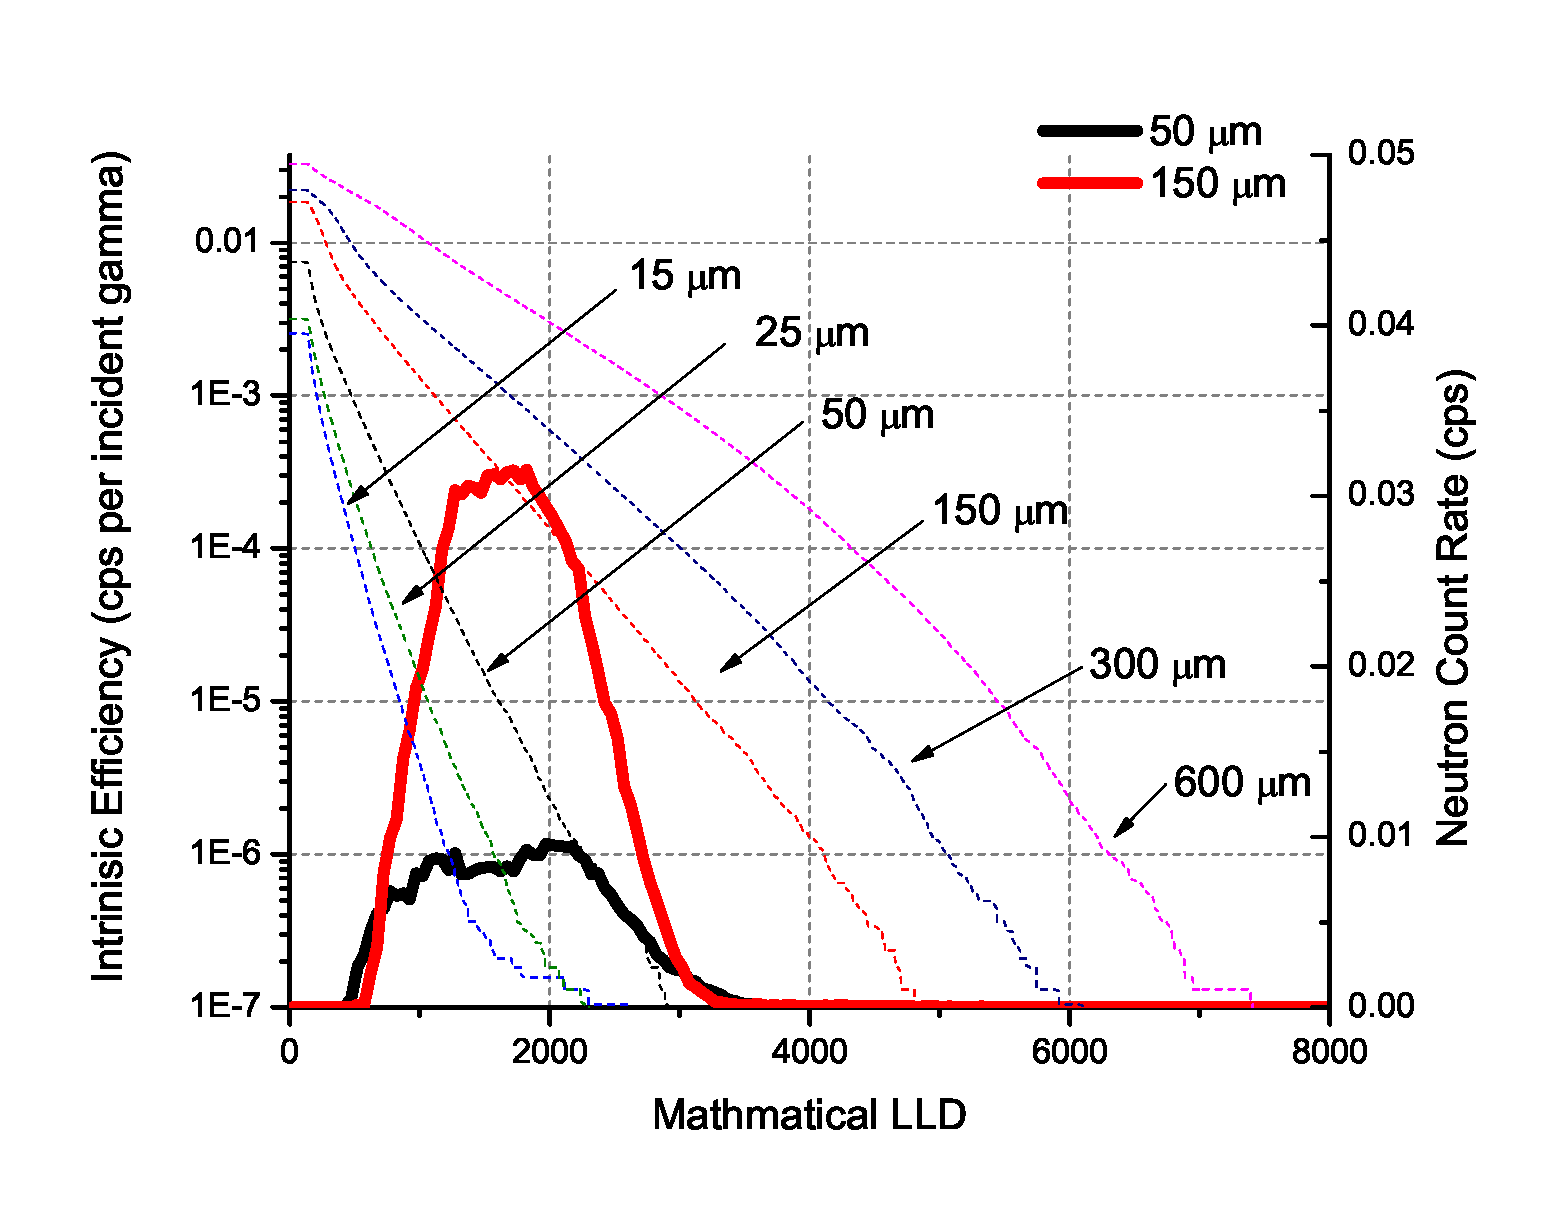
\includegraphics[width=\textwidth]{PS_IntEff_LiF20_PPO5}
    \caption[PS Gamma intrinsic efficiency and neutron count rate]{Gamma intrinsic efficiency (dashed lines) plotted against neutron counts (solid). The gamma spectra has been normalized by the number of incident photons upon the sample, while the neutron spectra has not.}
    \label{fig:GammaIntrNeutronCounts}
\end{figure}
\begin{figure}[ht]
    \centering
    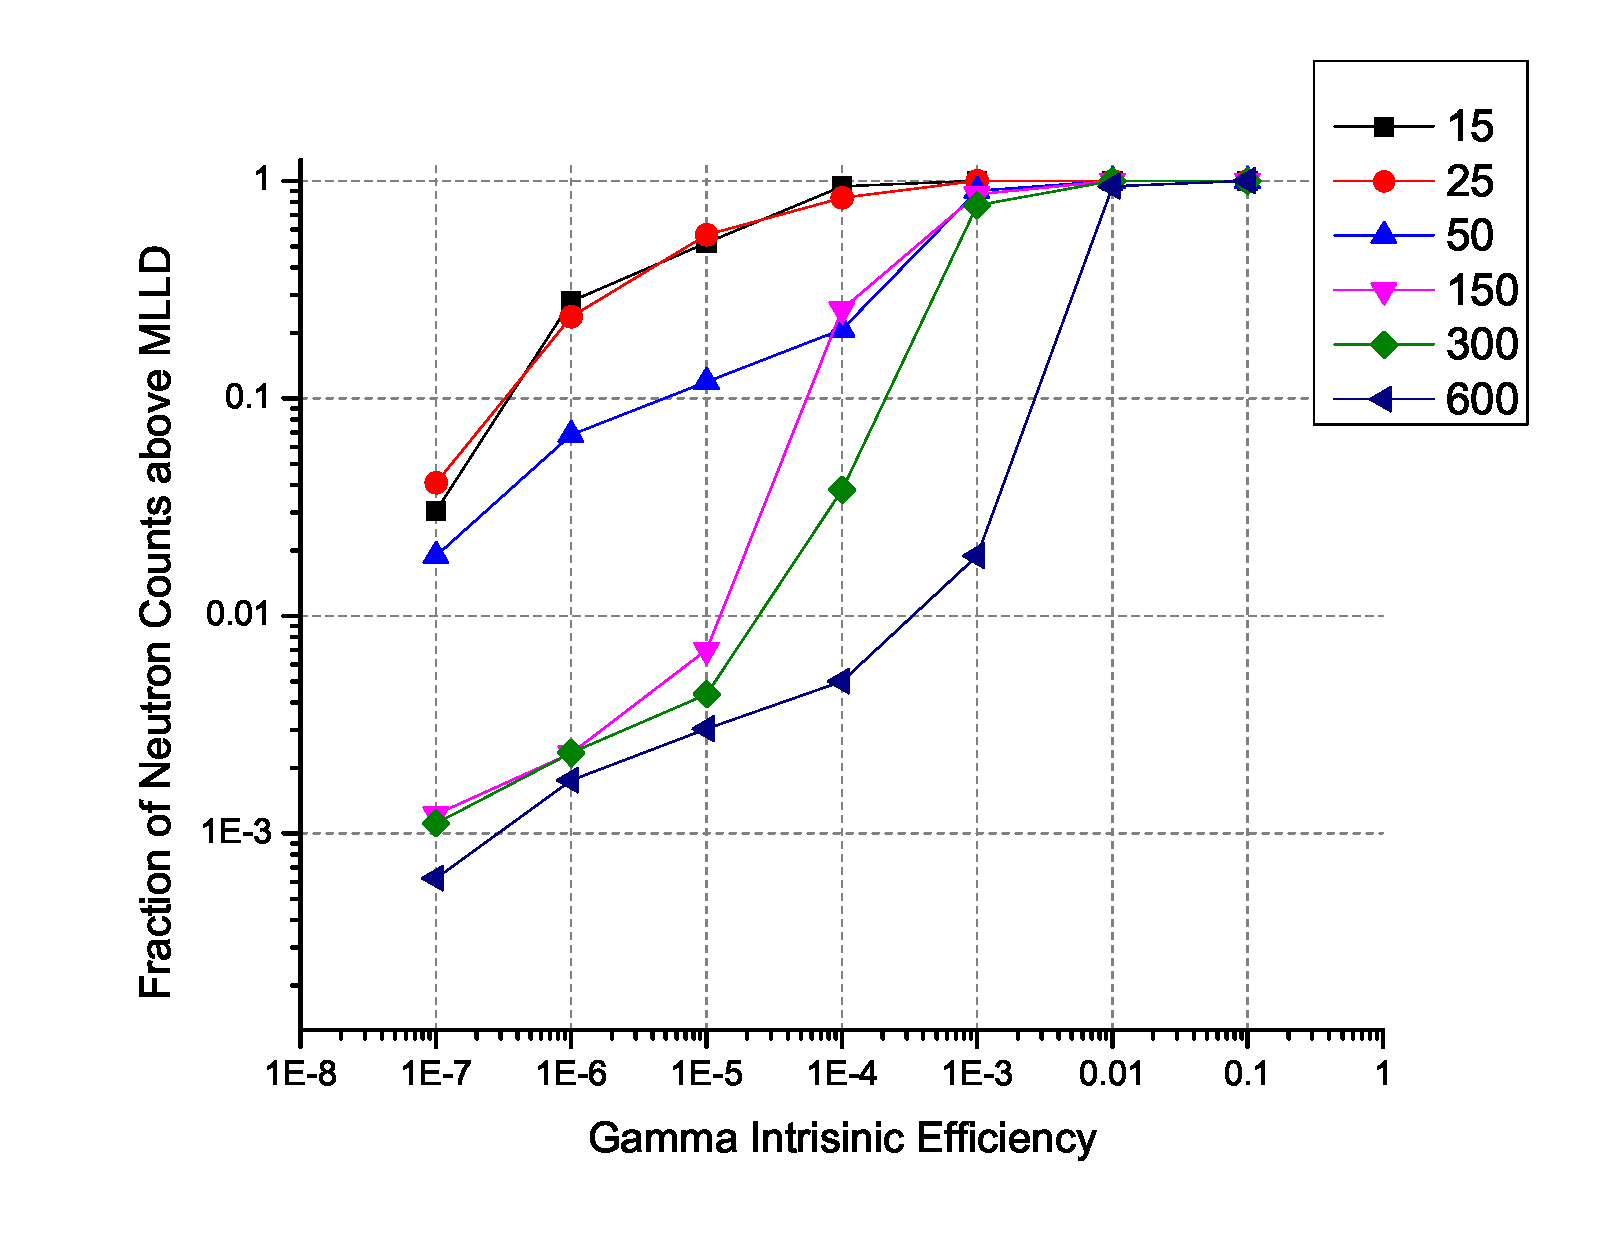
\includegraphics[width=\textwidth]{PS_IntFractionNCR_LiF}
    \caption{Intrinsic efficiency versus neutron count rate. }
    \label{fig:crVsIntEff}
\end{figure}
\begin{table}[]
    \caption{Fraction of Neutron Count Rate Above Discriminator Setting}
	\centering
	\begin{tabular}{c | c}
	Thickness & Neutron Fraction \\
	\hline
	\hline
	\SI{15}{\um} & 0.28 \\
	\SI{25}{\um} & 0.024 \\
	\SI{50}{\um}  & 0.067 \\
	\SI{150}{\um}  & 0.023 \\
	\SI{300}{\um}  & 0.023 \\
	\SI{600}{\um}  & 0.0017 \\
	\end{tabular}
  \label{tab:FractionCRGamma}
\end{table}
In addition it is observed in \autoref{fig:GammaIntrNeutronCounts} that for neutrons, thicker films only enhance the resolution of the film and do little to increase the light yield, as most of energy from a neutron event is captured in the film.
The average energy deposited was computed for each thickness and normalized by the incident energy for gammas by the Q-value of the reaction for neutrons, and is presented in Table ~\ref{tab:FractionEDep}.
For thickness greater than \SI{150}{\um} there is little benefit in increasing the thickness of the film in terms of energy deposition by neutrons, since over 90\% of the energy is being deposited in the film.
\begin{table}[ht]
    \caption{Fractional Energy Deposition for Various Thickness}
	\centering
	\begin{tabular}{c | c c}
	Thickness & Gamma Fraction & Neutron Fraction \\
	\hline
	\hline
	\SI{15}{\um} & 0.010 & 0.531 \\
	\SI{25}{\um} & 0.013 & 0.634 \\
	\SI{50}{\um} & 0.017 & 0.782 \\
	\SI{150}{\um} & 0.032 & 0.927 \\
	\SI{300}{\um} & 0.052 & 0.964 \\
	\SI{600}{\um} & 0.087 & 0.982 \\
	\SI{1}{\mm} & 0.130 & 0.989 \\
	\SI{1}{\cm} & 0.425 & 0.998 \\
	\end{tabular}
  \label{tab:FractionEDep}
\end{table}

